\label{chap:lit_review}
\chapter{Literature review}
\section{Preface}

This chapter consists of a literature review which discusses the evolutionary dynamics of bacterial small non-coding RNAs (sRNAs). In this review we discuss possible explanations for observed gain and loss of sRNAs over short evolutionary timescales, focusing on the mechanisms and rates by which these genes might originate and diversify. We consider the potential for bacterial genomes to generate and remove \textit{de novo} genes by insertion and deletion events, recombination, or by the capture of a pool of stochastically-arising transcripts, termed "transcriptional noise". Examples of sRNA acquisition \textit{via} exaptation, duplication and diversification, and horizontal gene transfer are also reviewed. We outline the selection pressures expected to act on each of these routes, the evidence supporting such events and their relative probabilities.

This chapter is published as follows:
Bethany R. Jose, Paul P. Gardner, Lars Barquist; Transcriptional noise and exaptation as sources for bacterial sRNAs. Biochem Soc Trans 30 April 2019; 47 (2): 527–539. doi: https://doi.org/10.1042/BST20180171

\subsection{Contributions}
Lars Barquist and I produced the final version of the manuscript. I wrote the initial drafts of the manuscript, and generated all figures.  Lars Barquist and Paul Gardner developed the drake equation shown in Figure 4A.
\newpage
\begin{figure}
    \centering
    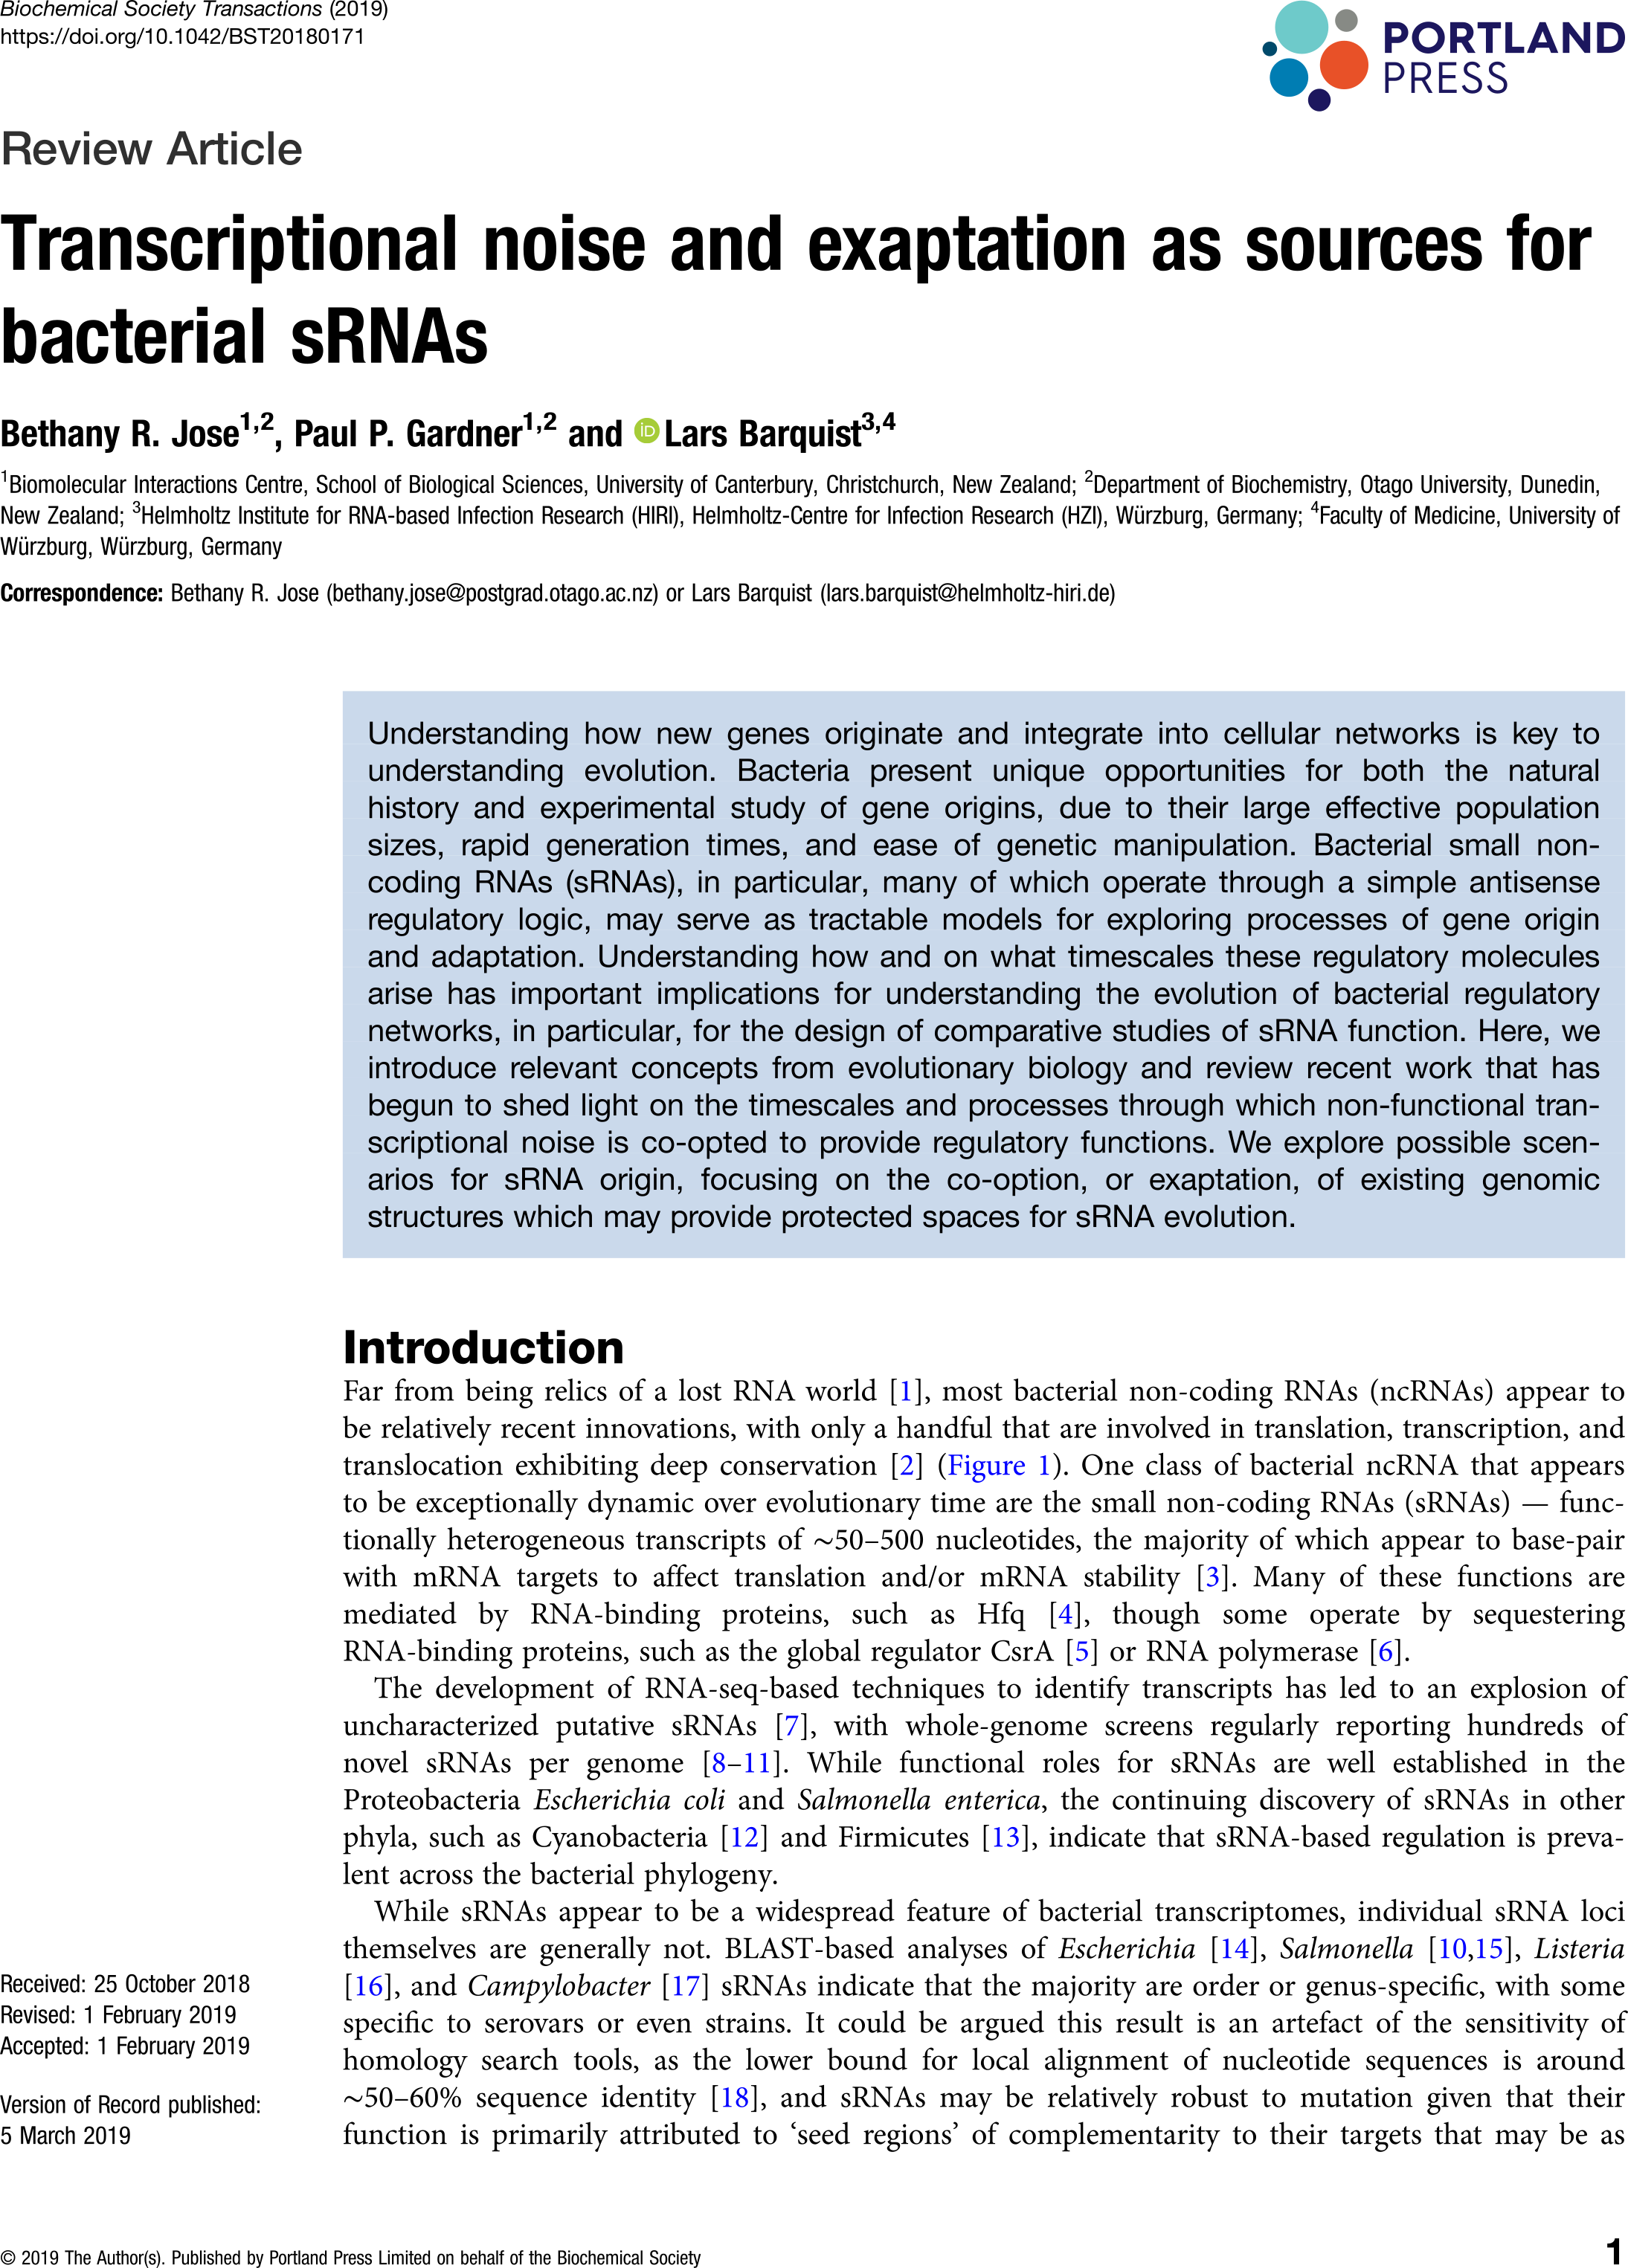
\includegraphics[width=\linewidth]{lit_review/page1.png}
\end{figure}
\begin{figure}
    \centering
    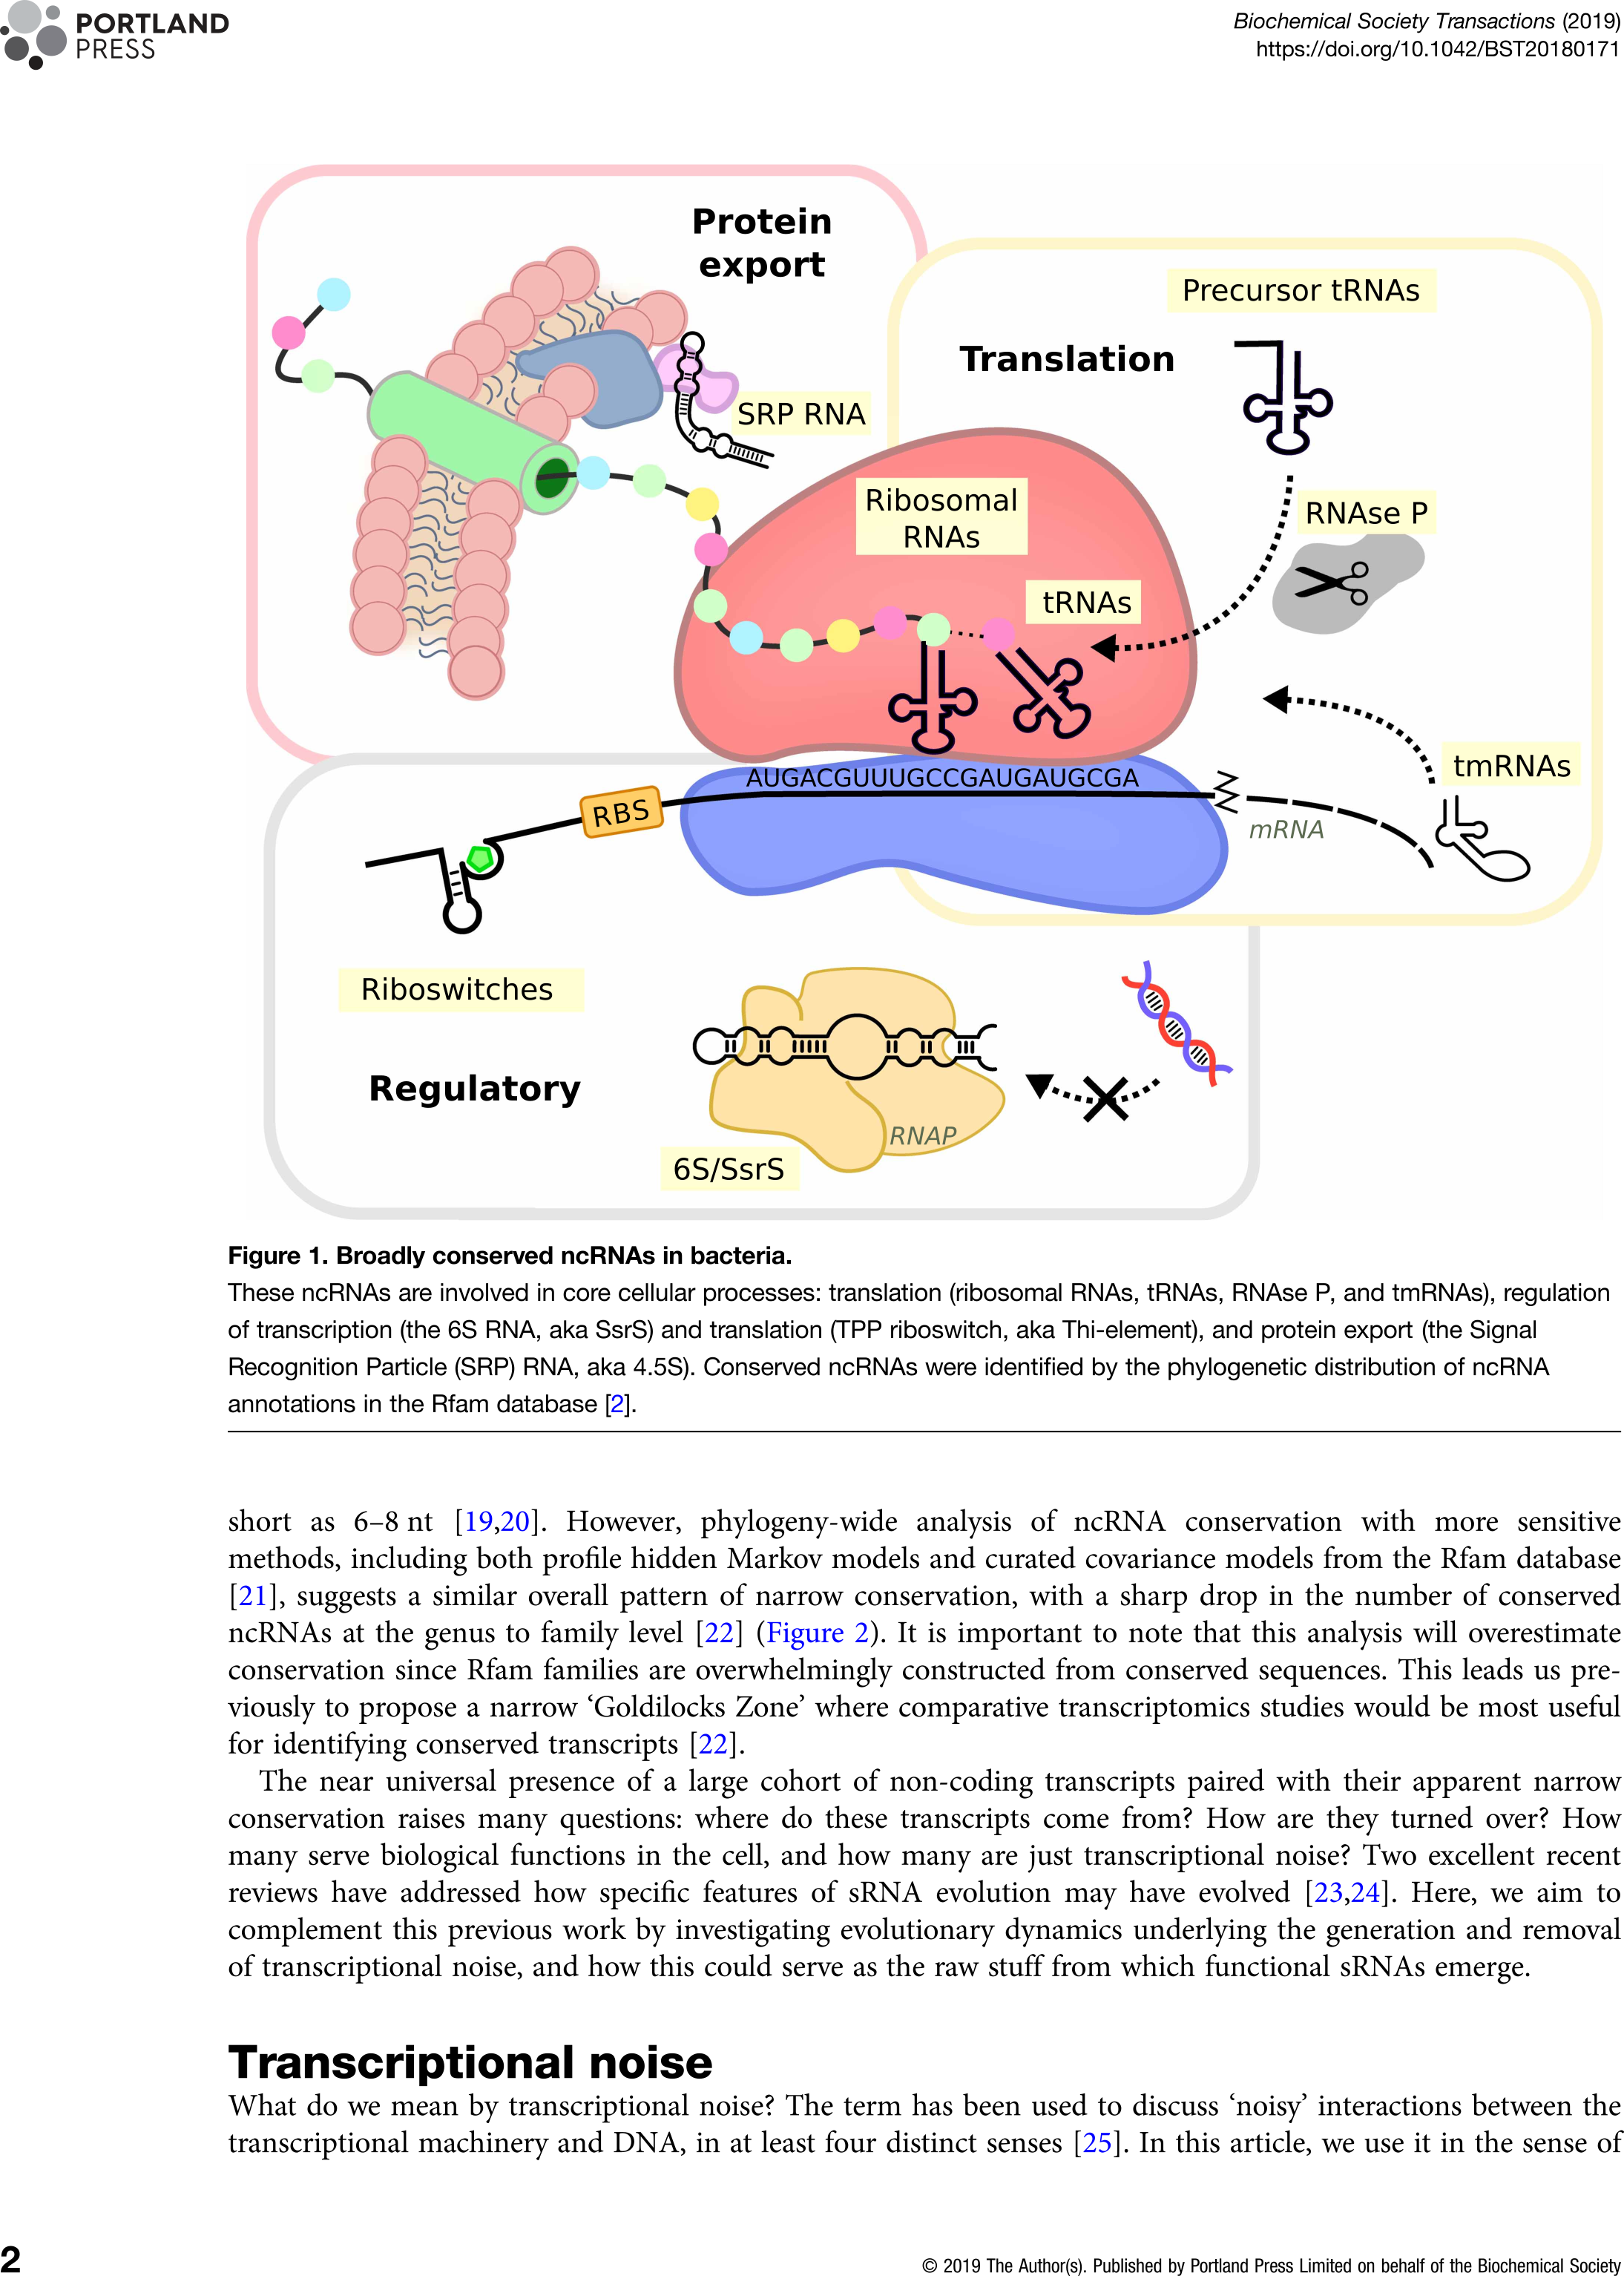
\includegraphics[width=\linewidth]{lit_review/page2.png}
\end{figure}
\begin{figure}
    \centering
    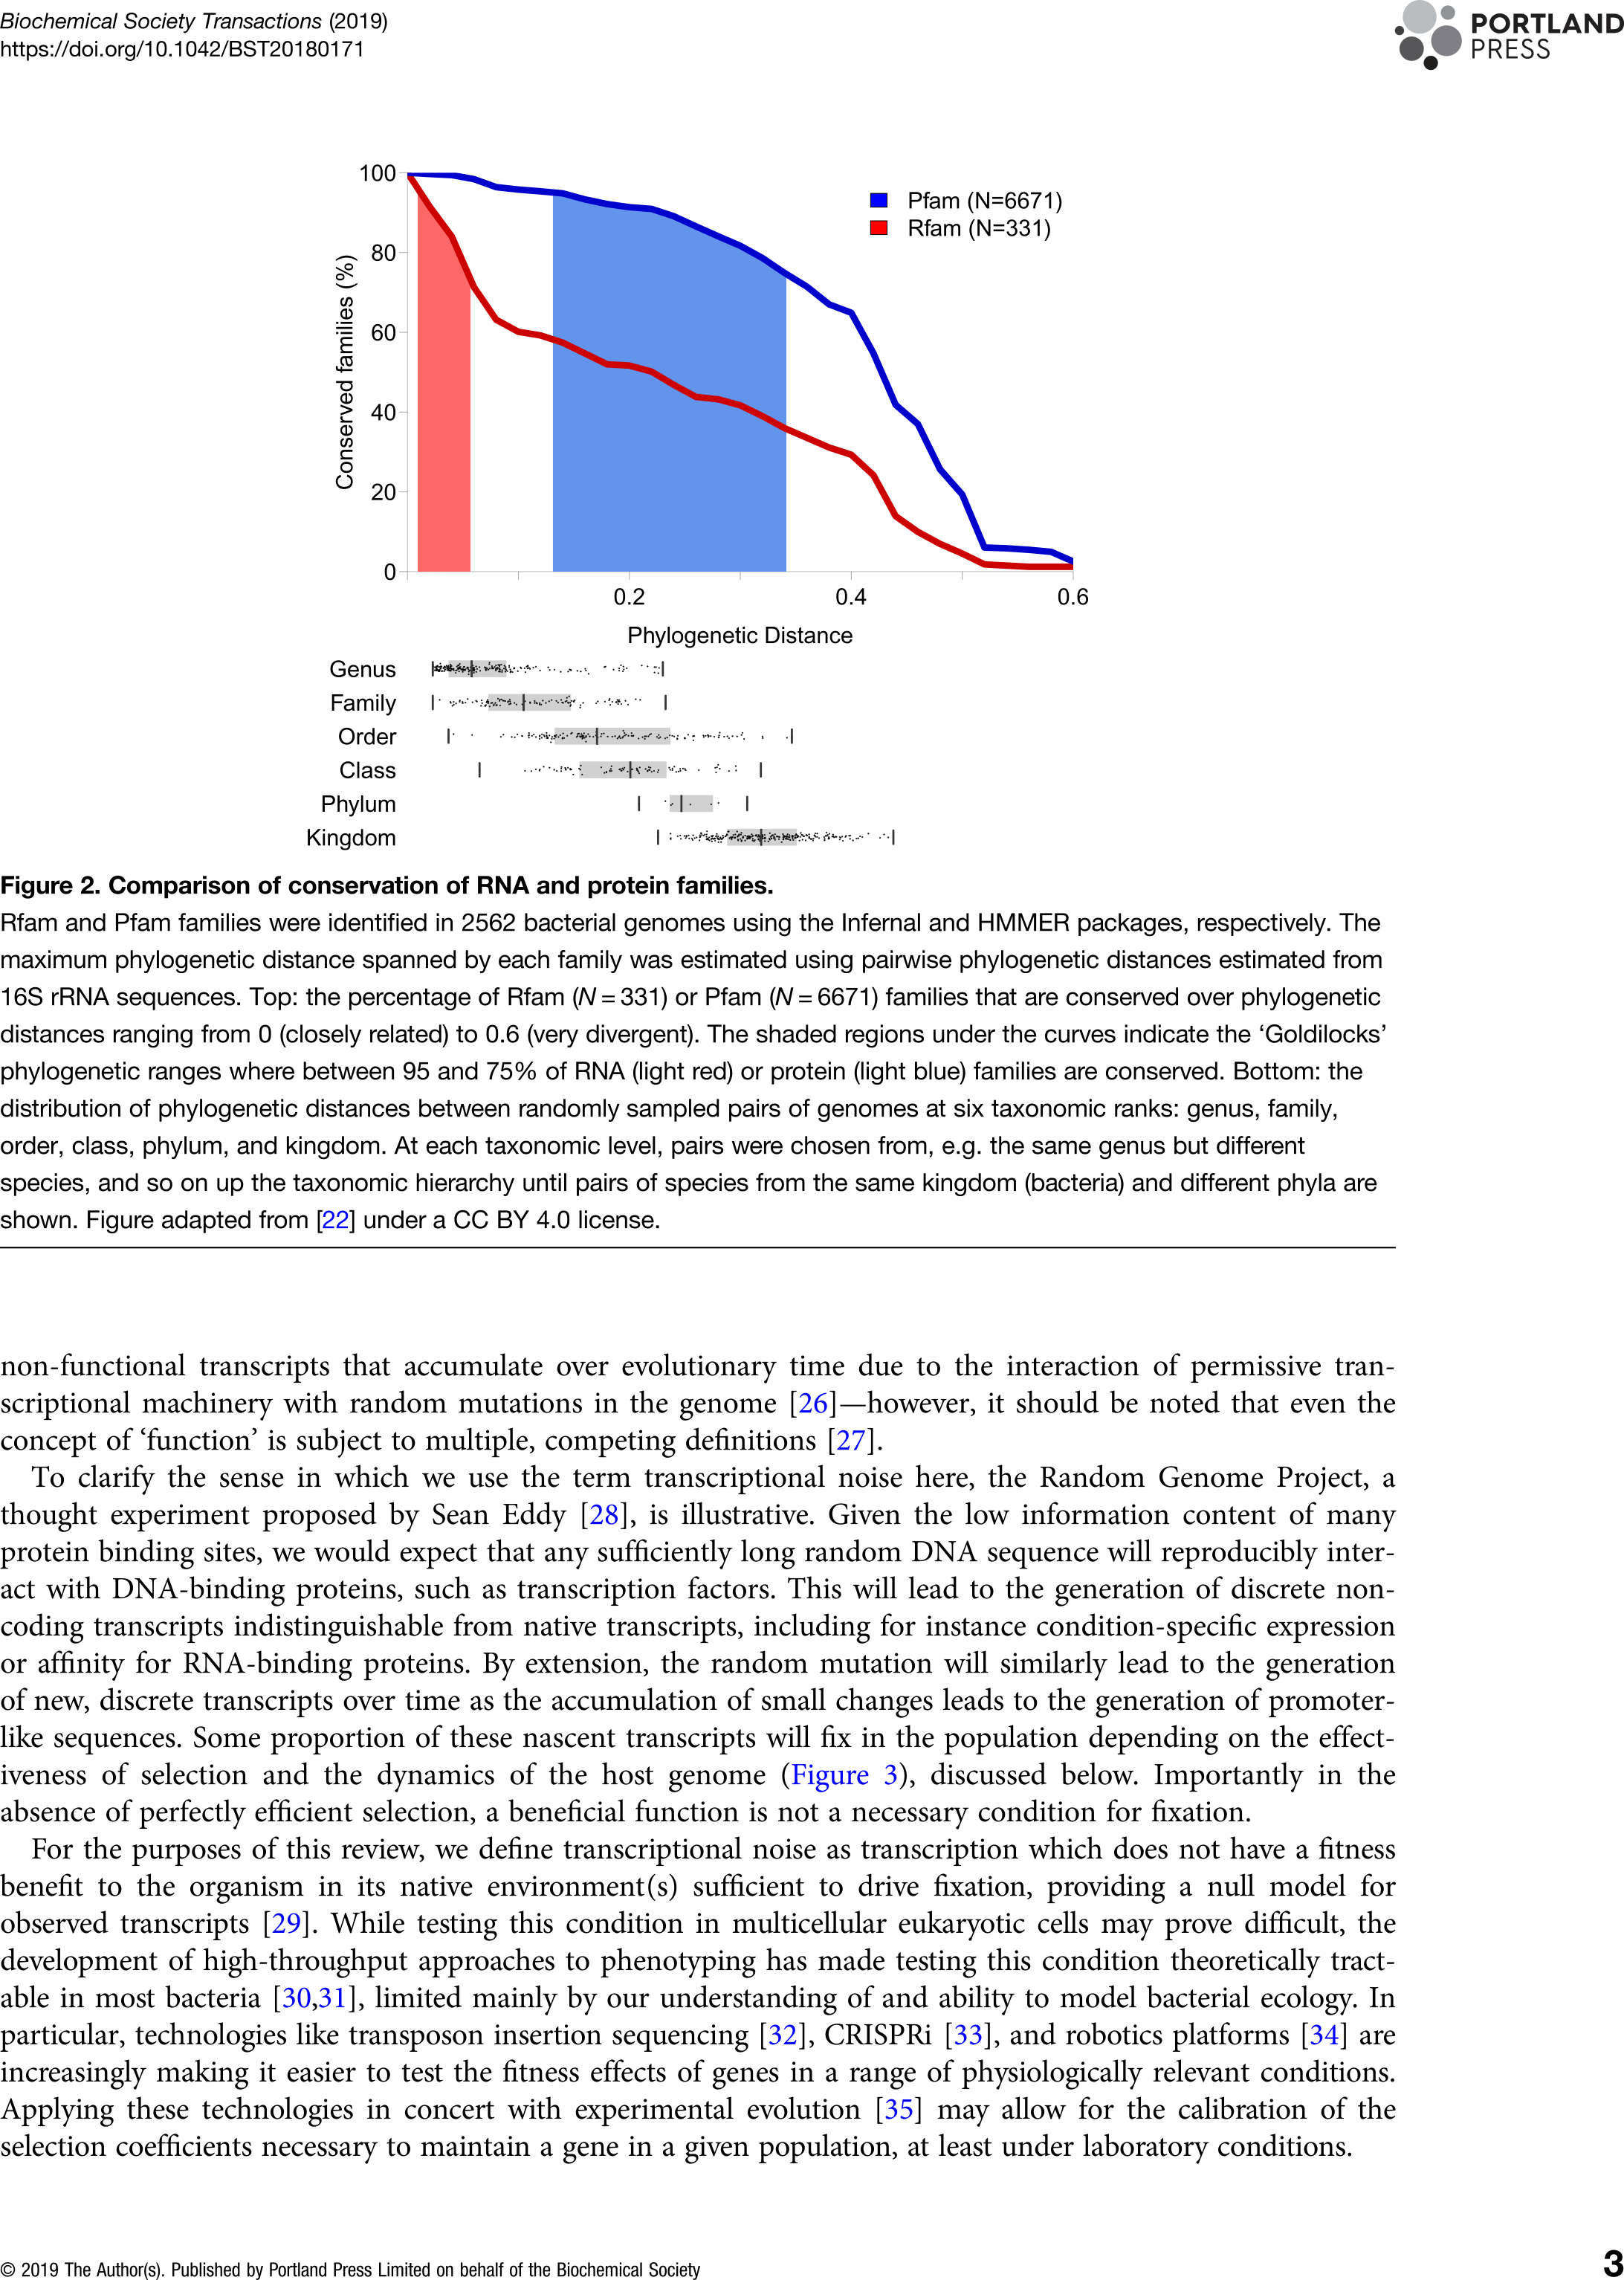
\includegraphics[width=\linewidth]{lit_review/page3.png}
\end{figure}
\begin{figure}
    \centering
    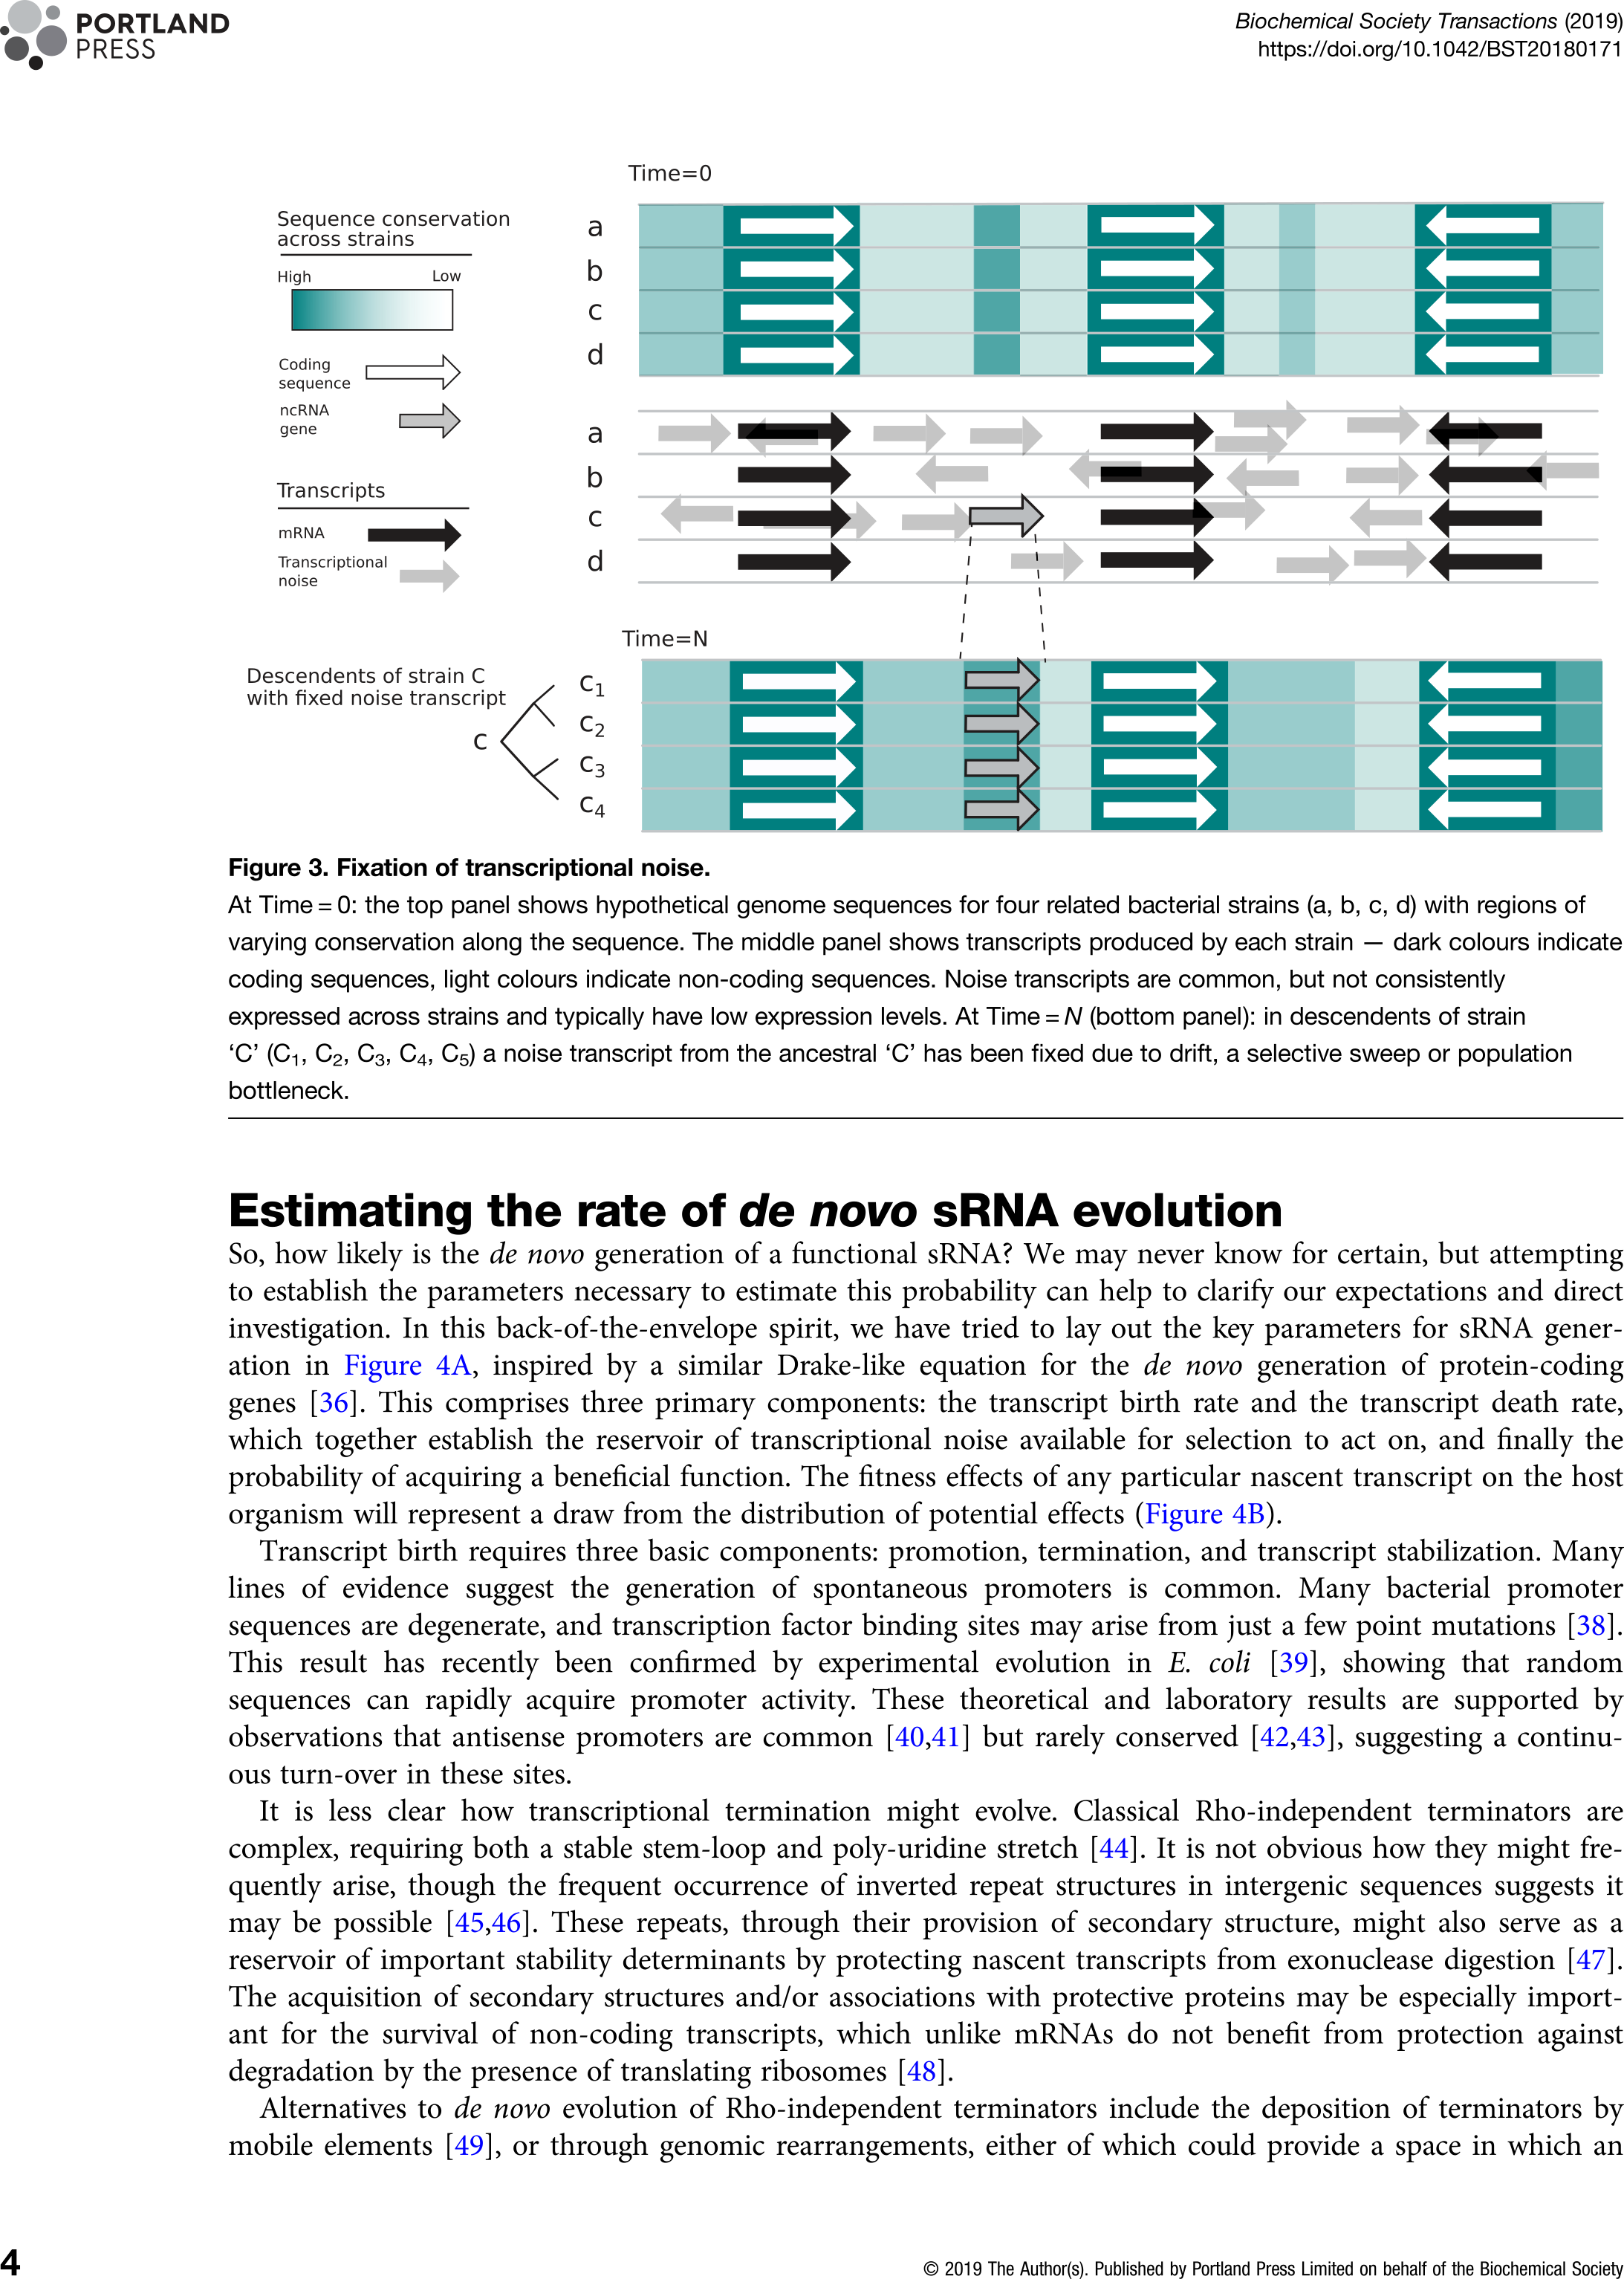
\includegraphics[width=\linewidth]{lit_review/page4.png}
\end{figure}
\begin{figure}
    \centering
    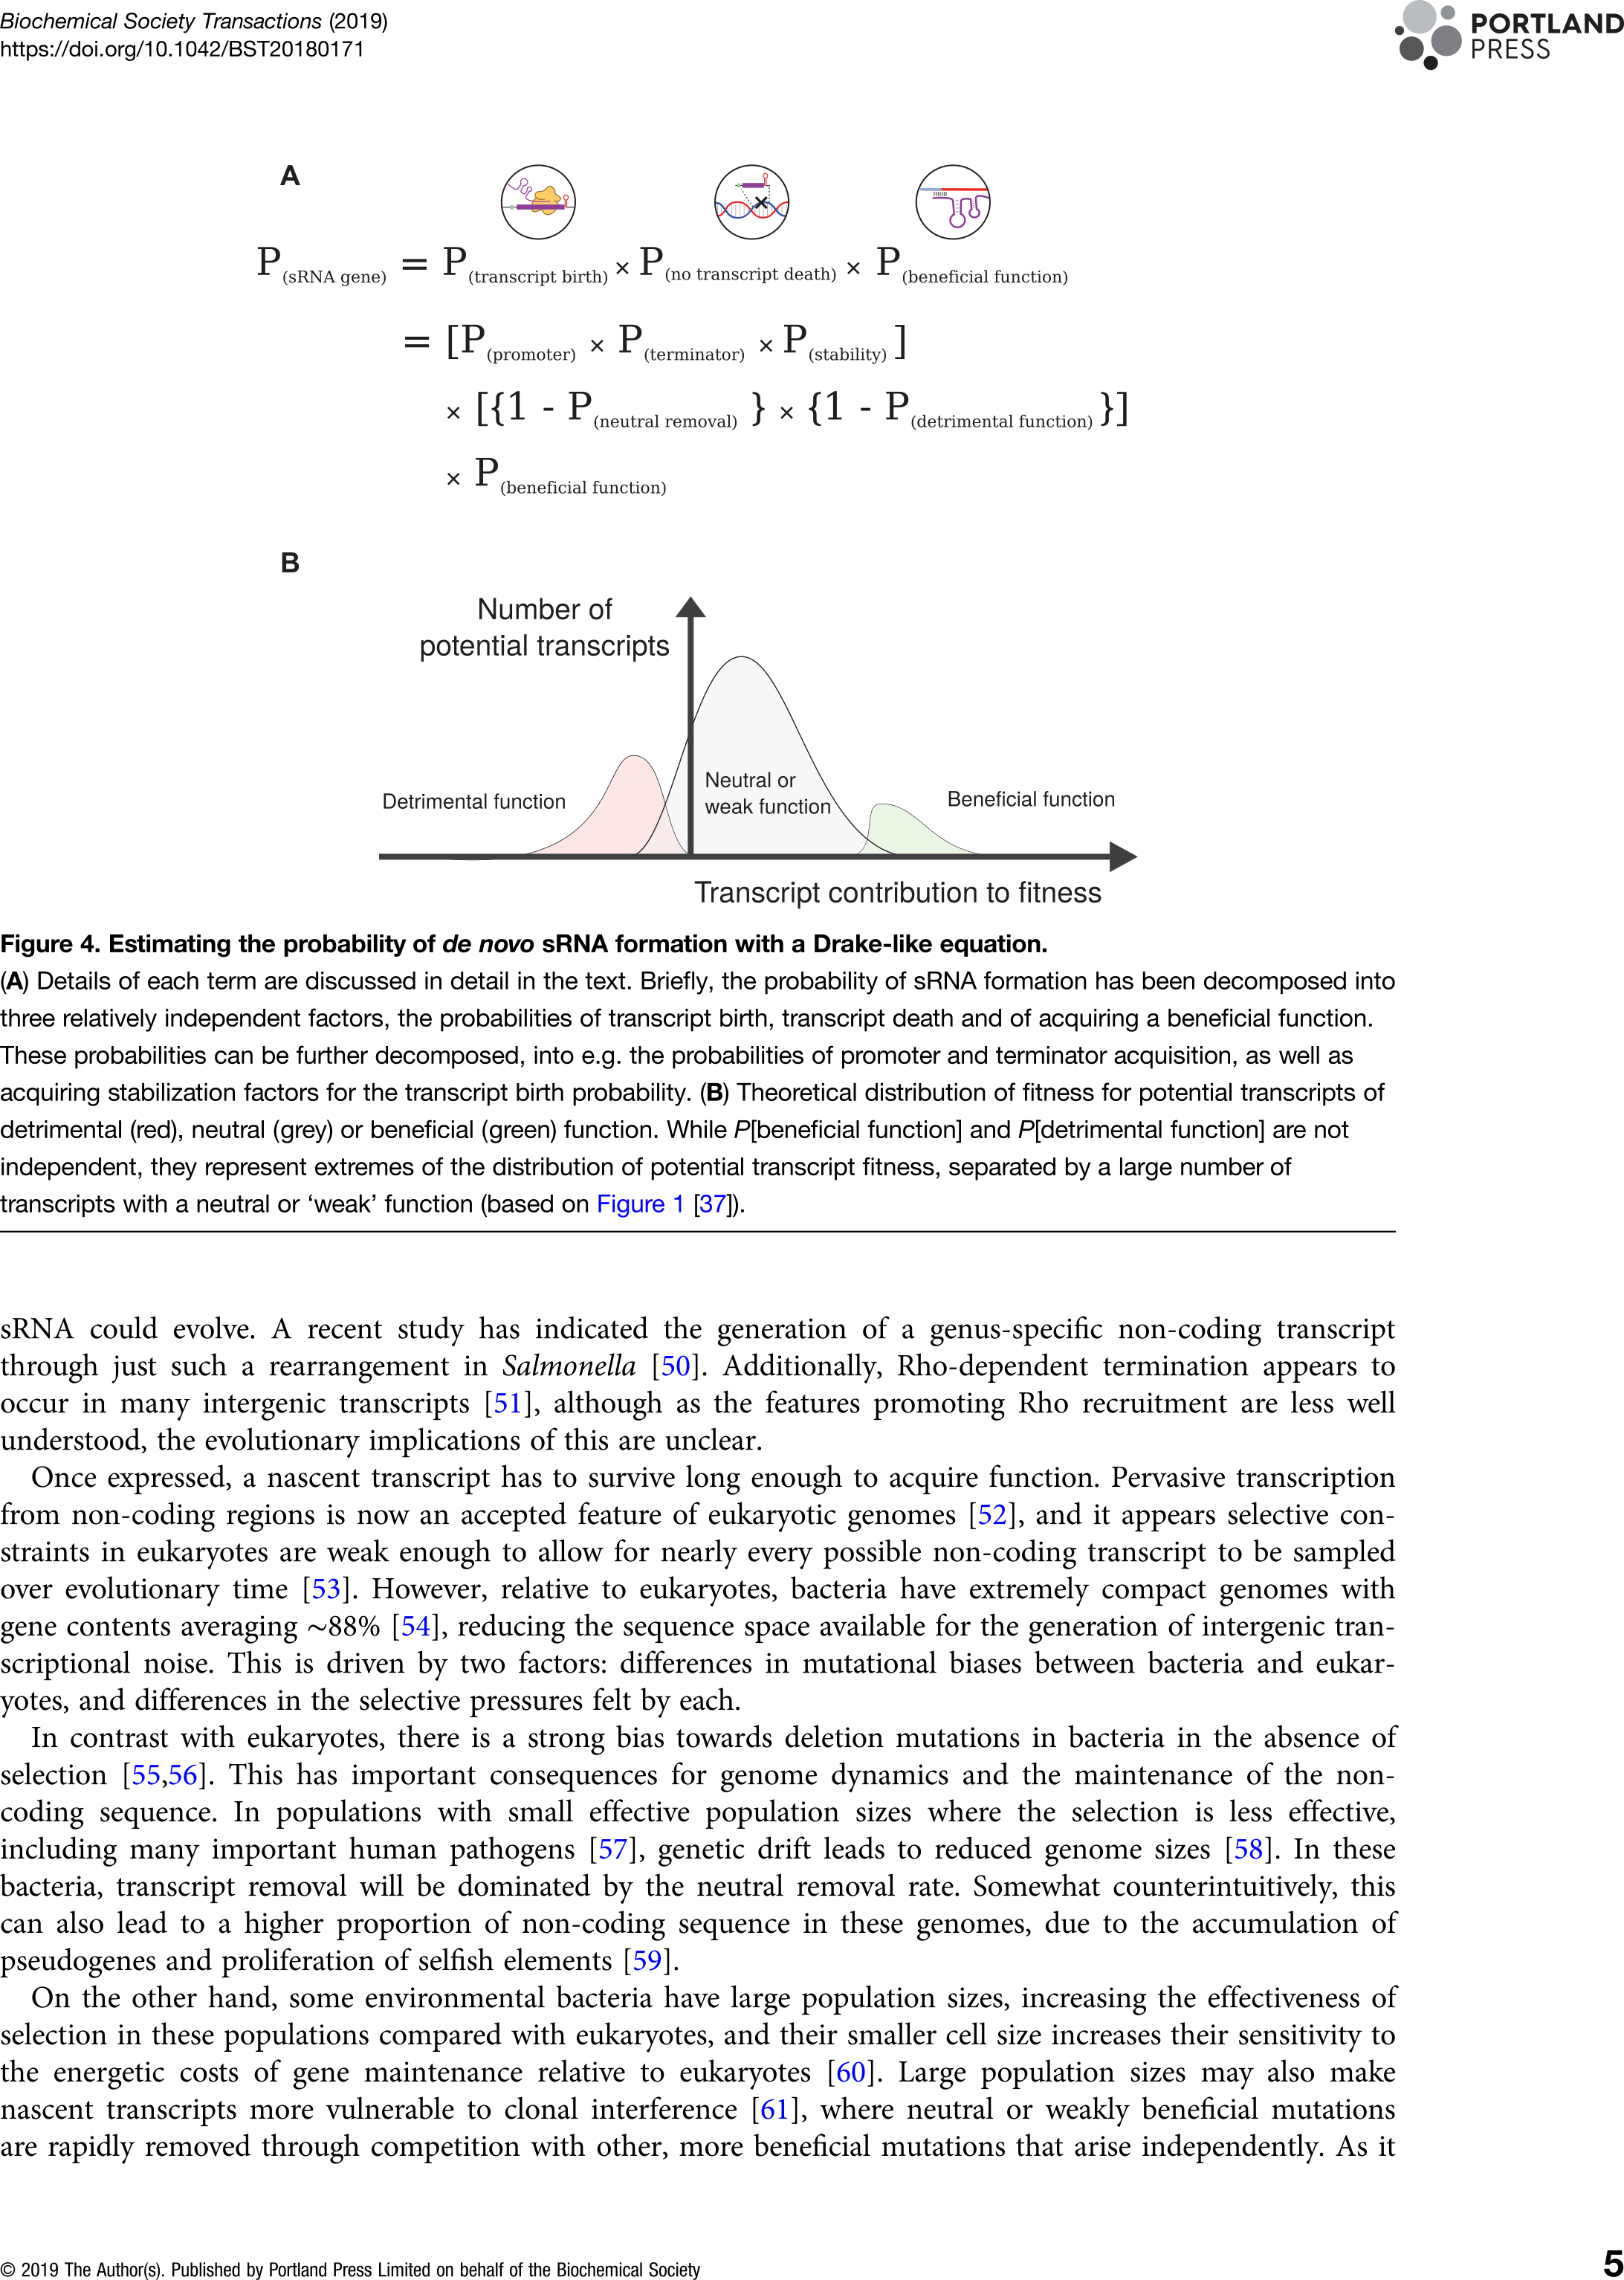
\includegraphics[width=\linewidth]{lit_review/page5.png}
\end{figure}
\begin{figure}
    \centering
    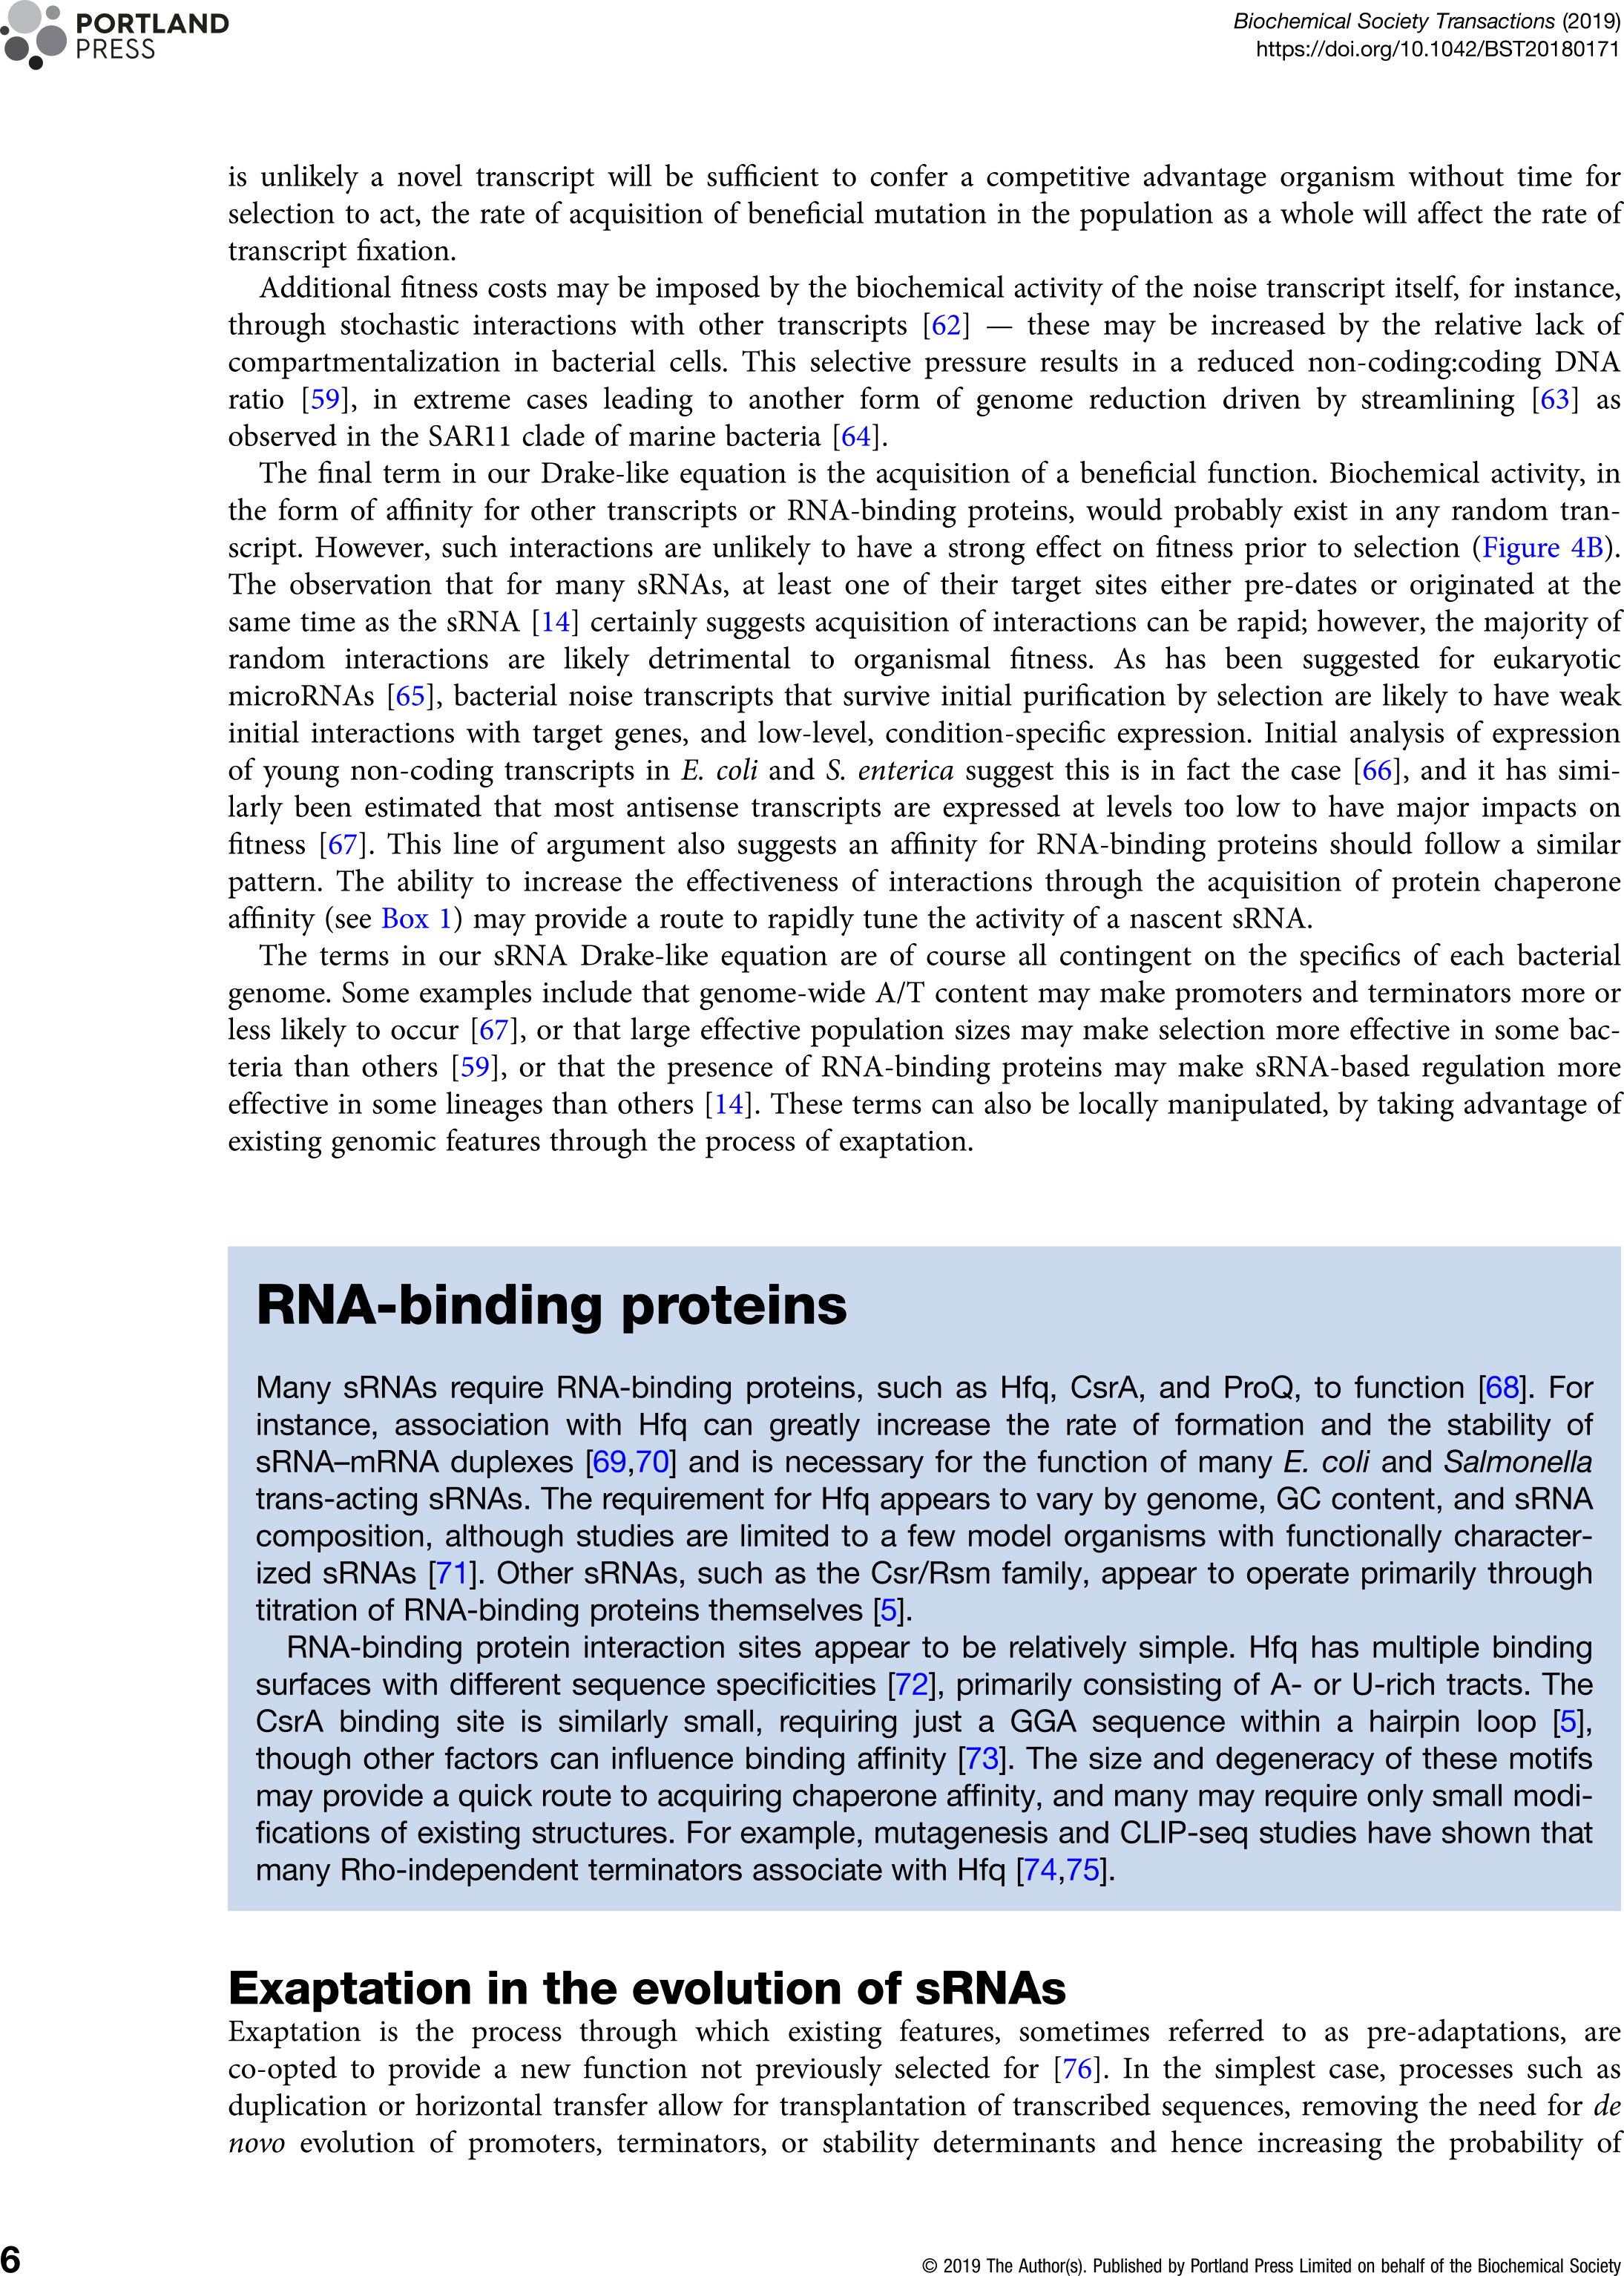
\includegraphics[width=\linewidth]{lit_review/page6.png}
\end{figure}
\begin{figure}
    \centering
    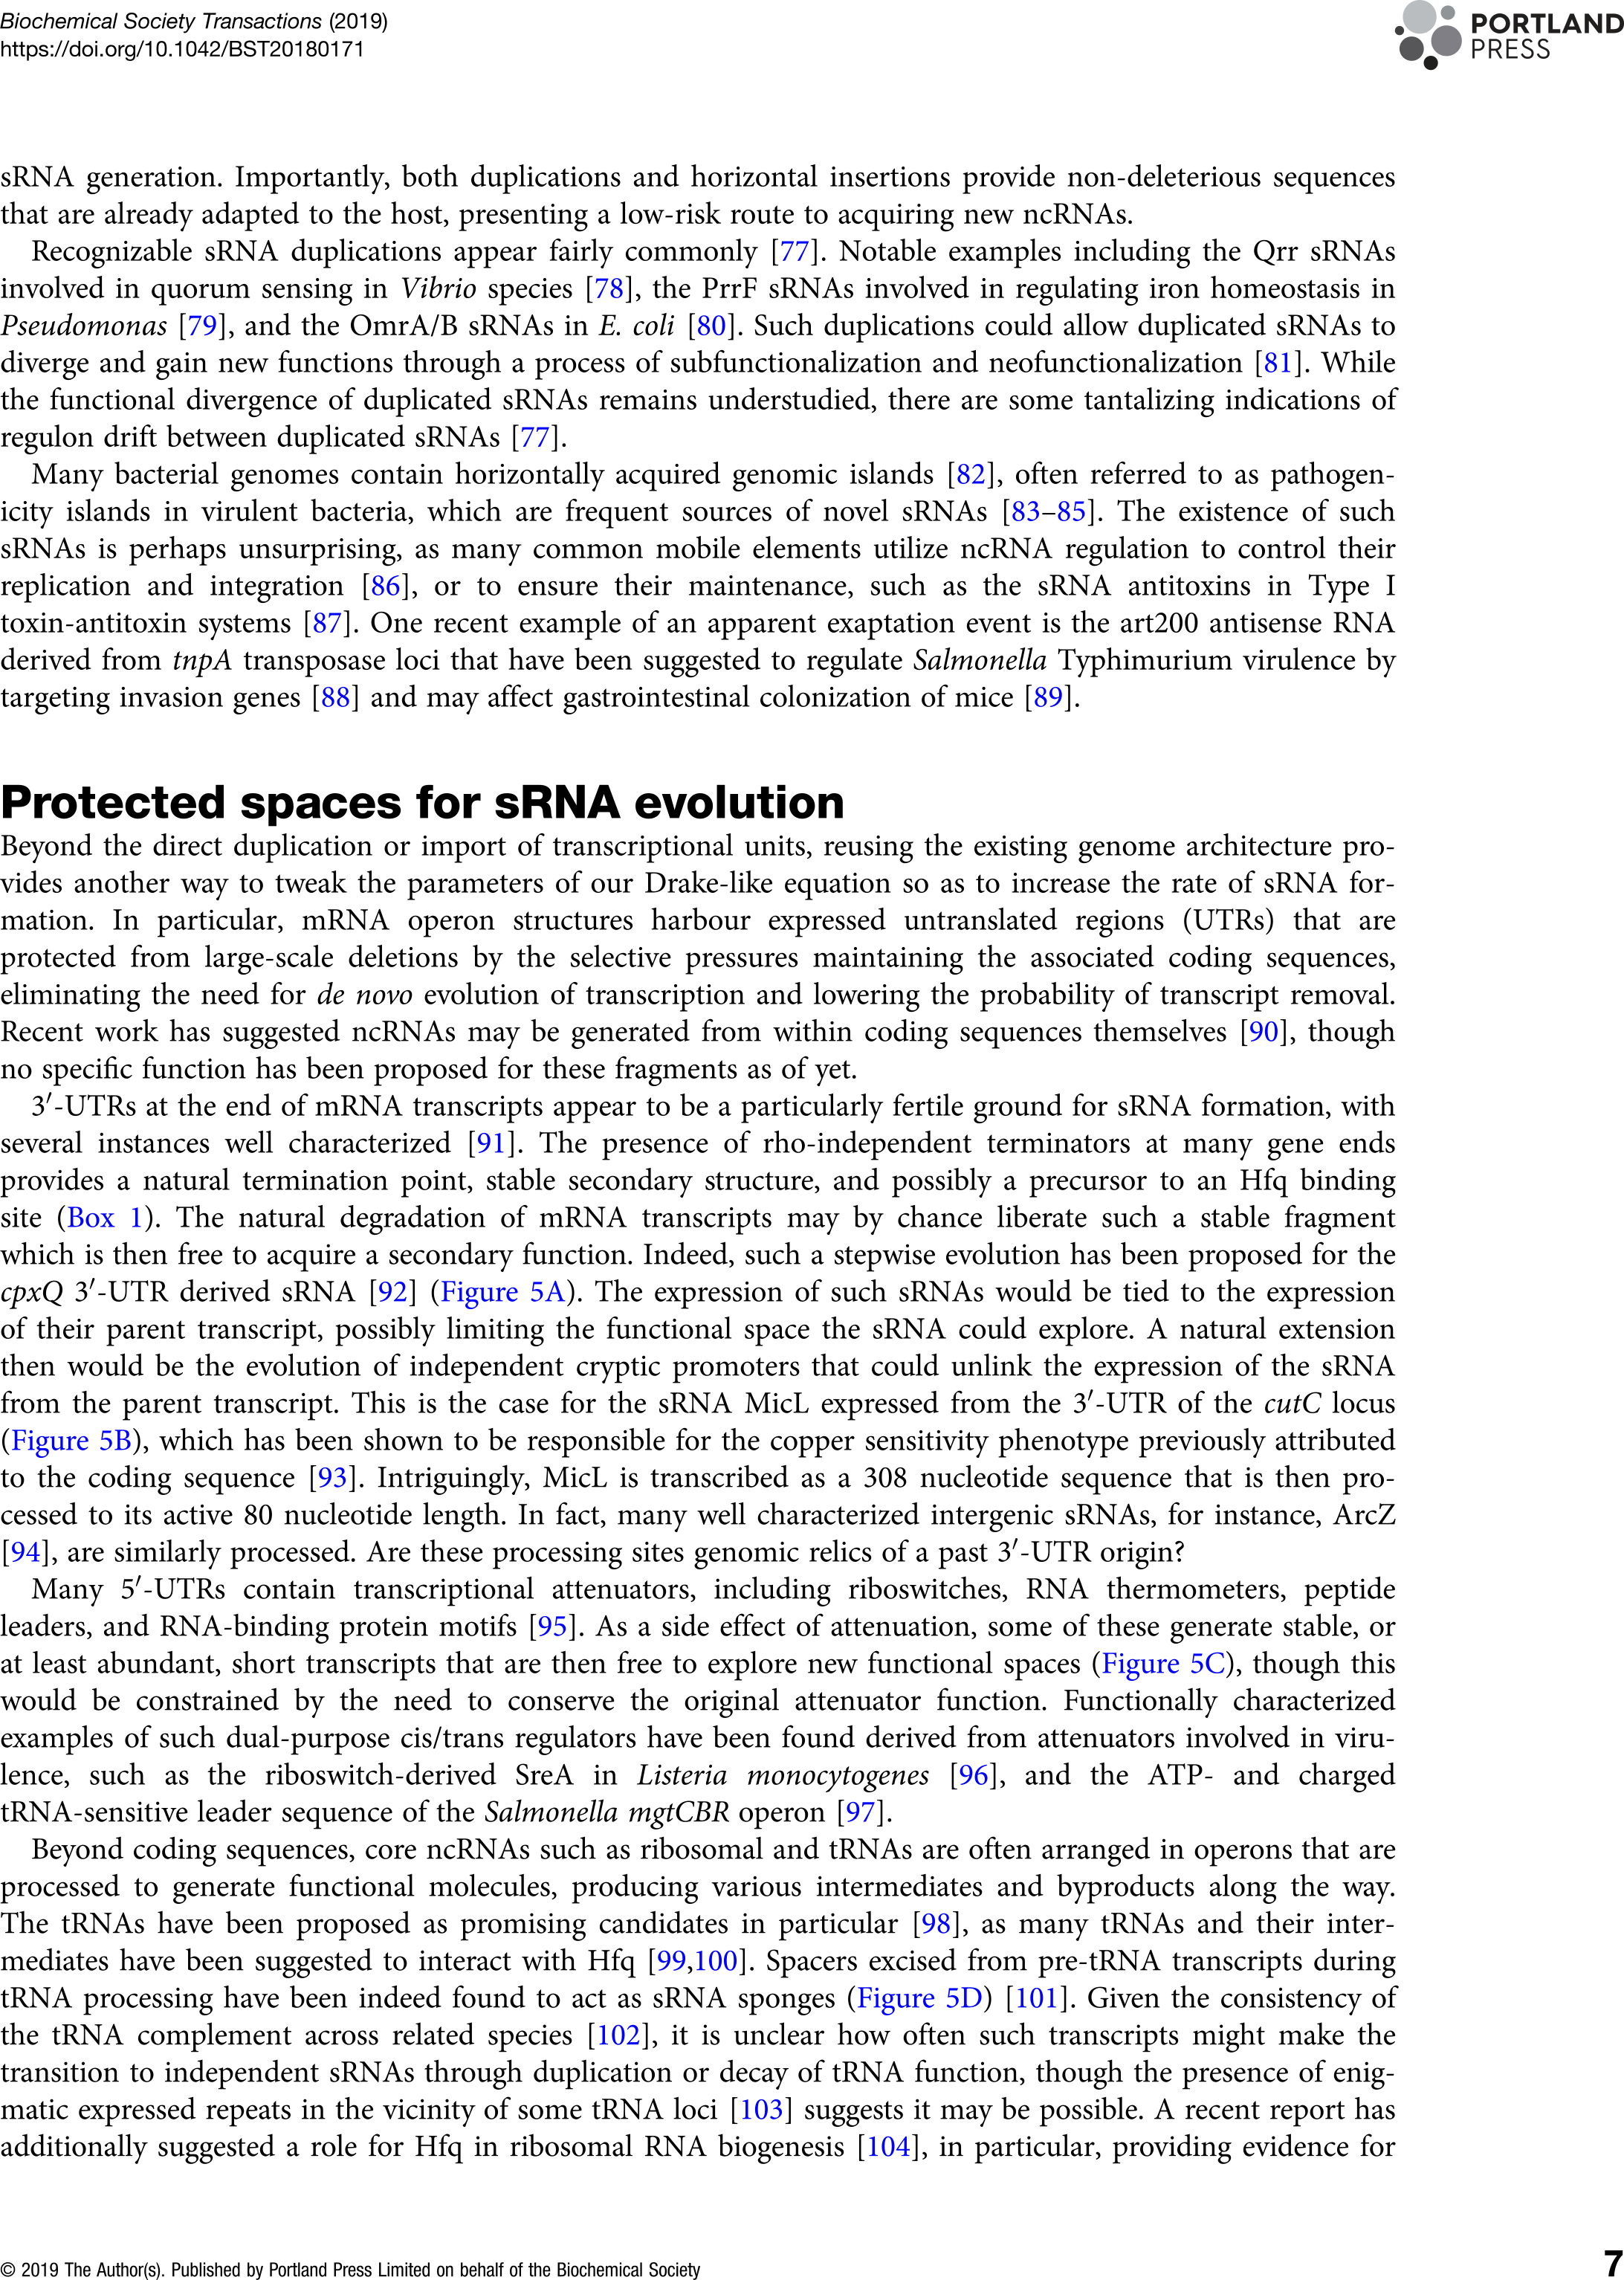
\includegraphics[width=\linewidth]{lit_review/page7.png}
\end{figure}
\begin{figure}
    \centering
    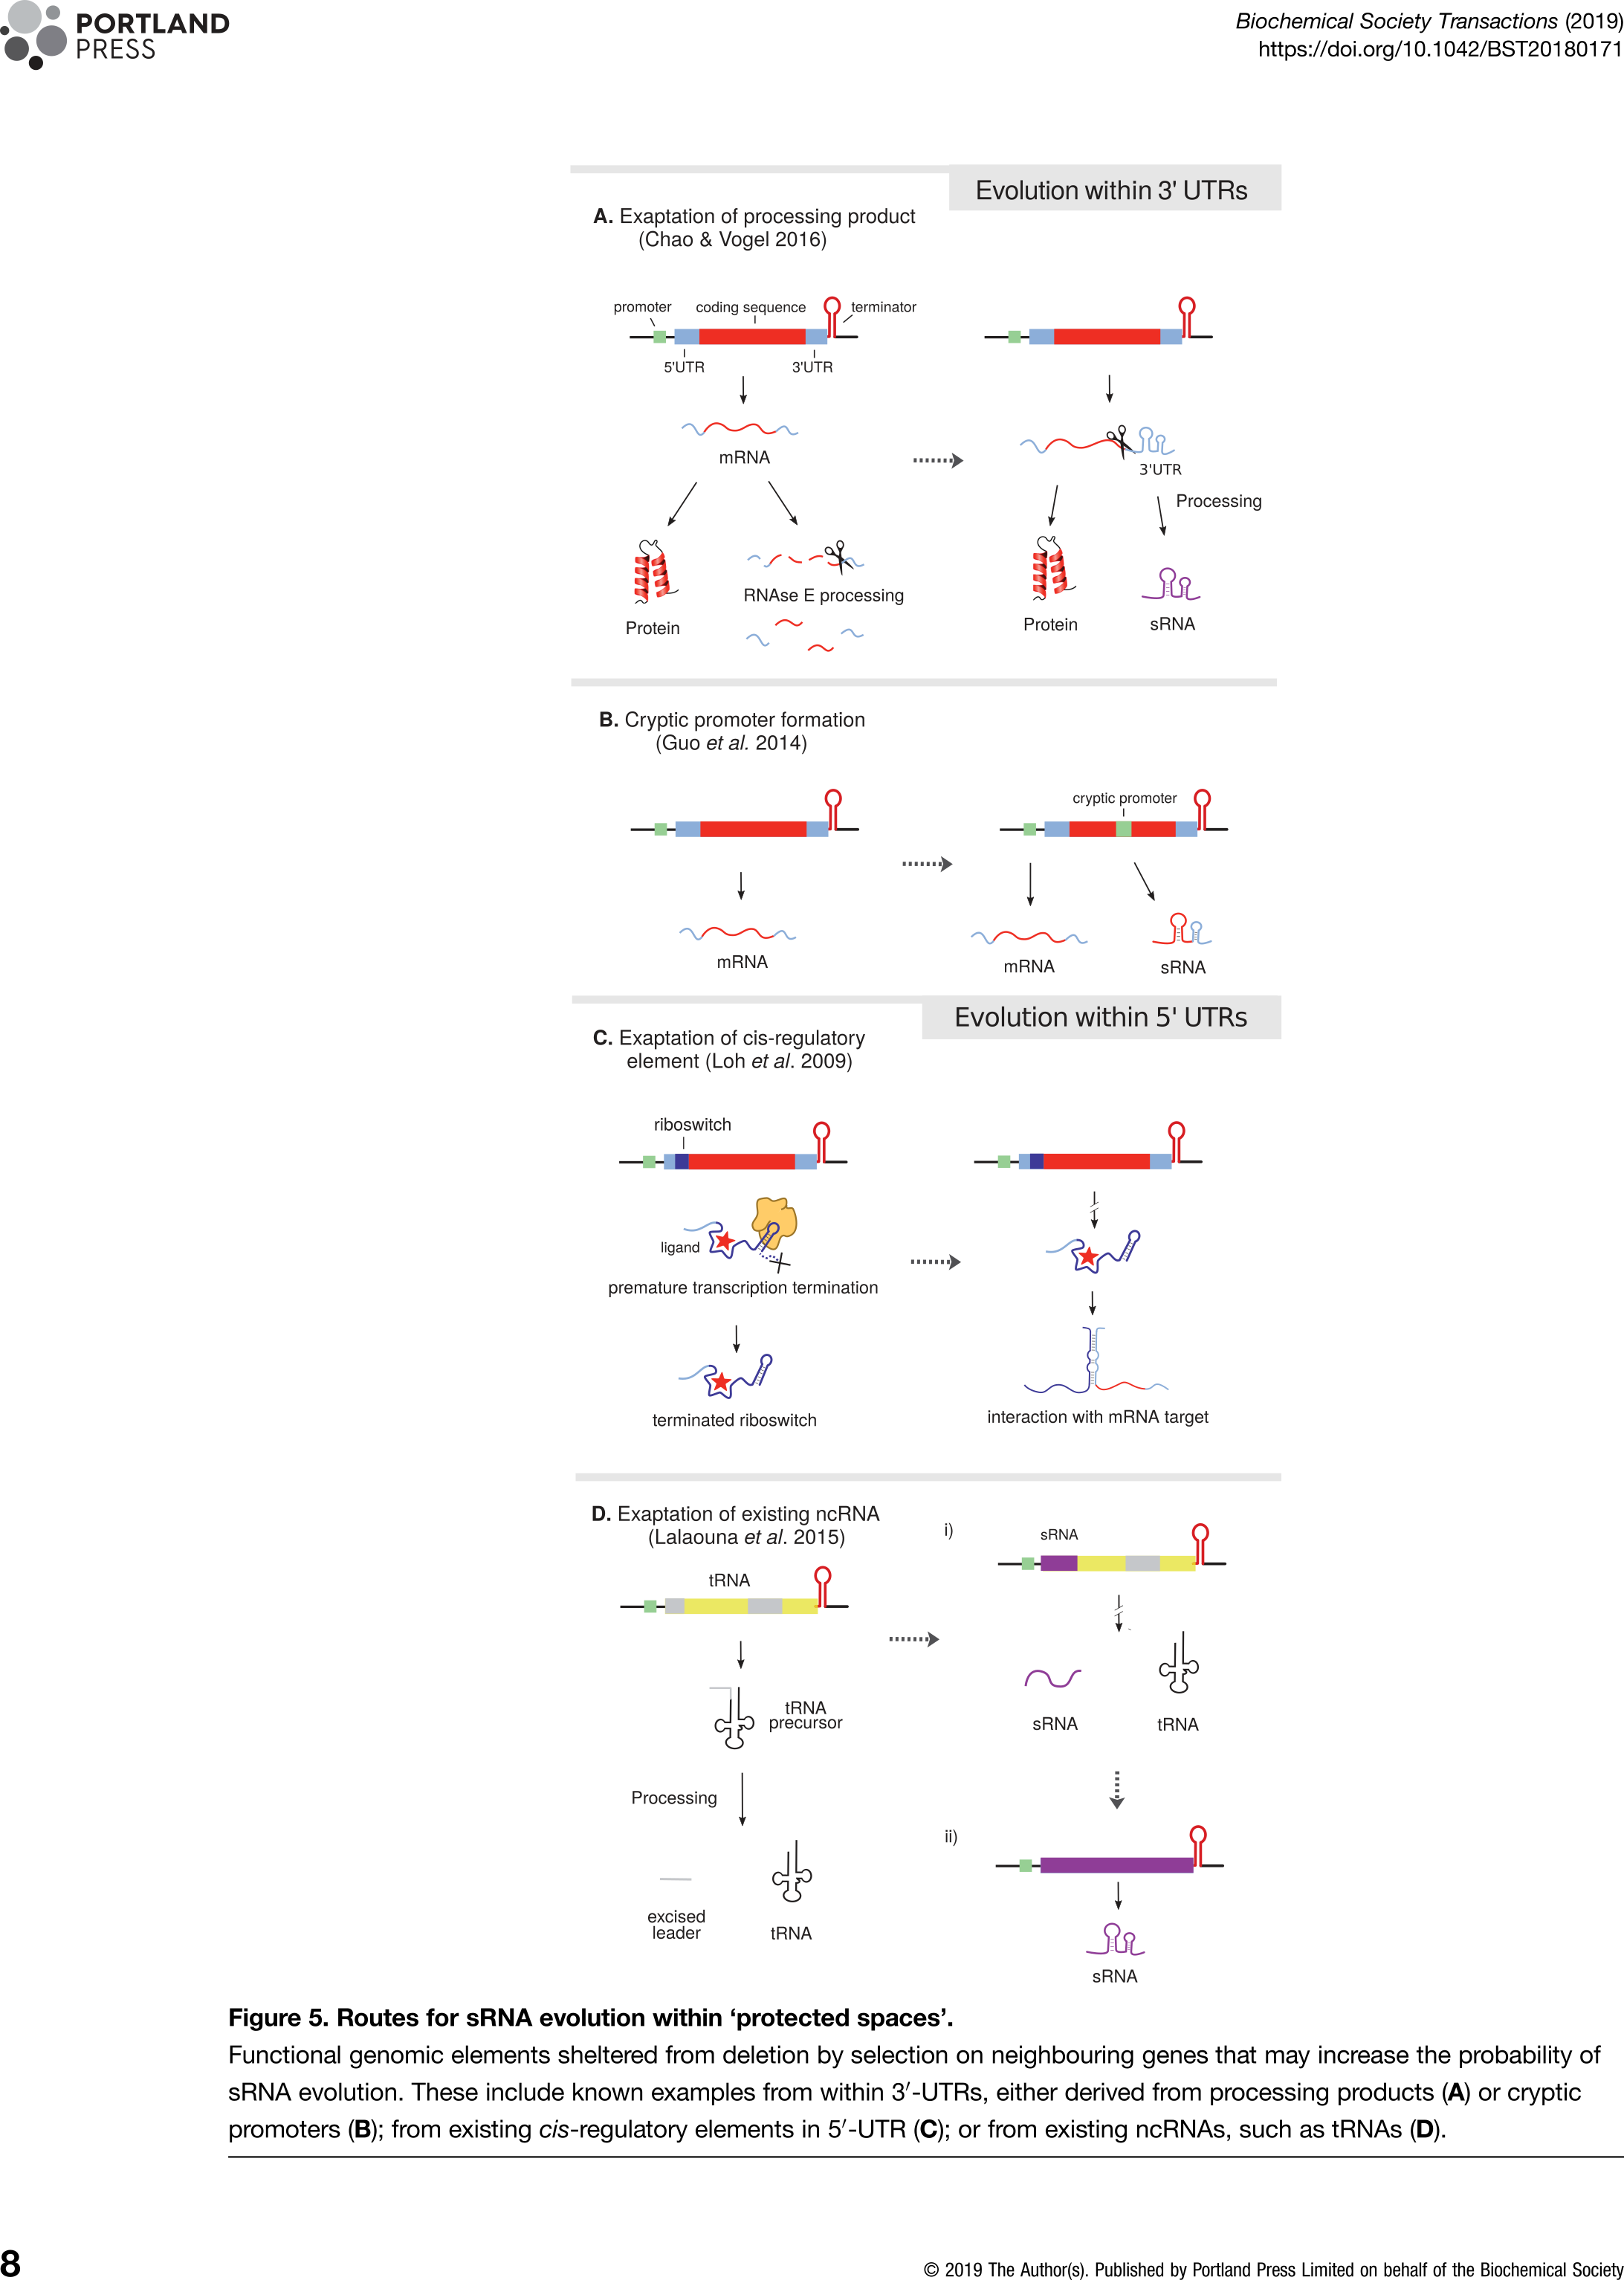
\includegraphics[width=\linewidth]{lit_review/page8.png}
\end{figure}
\begin{figure}
    \centering
    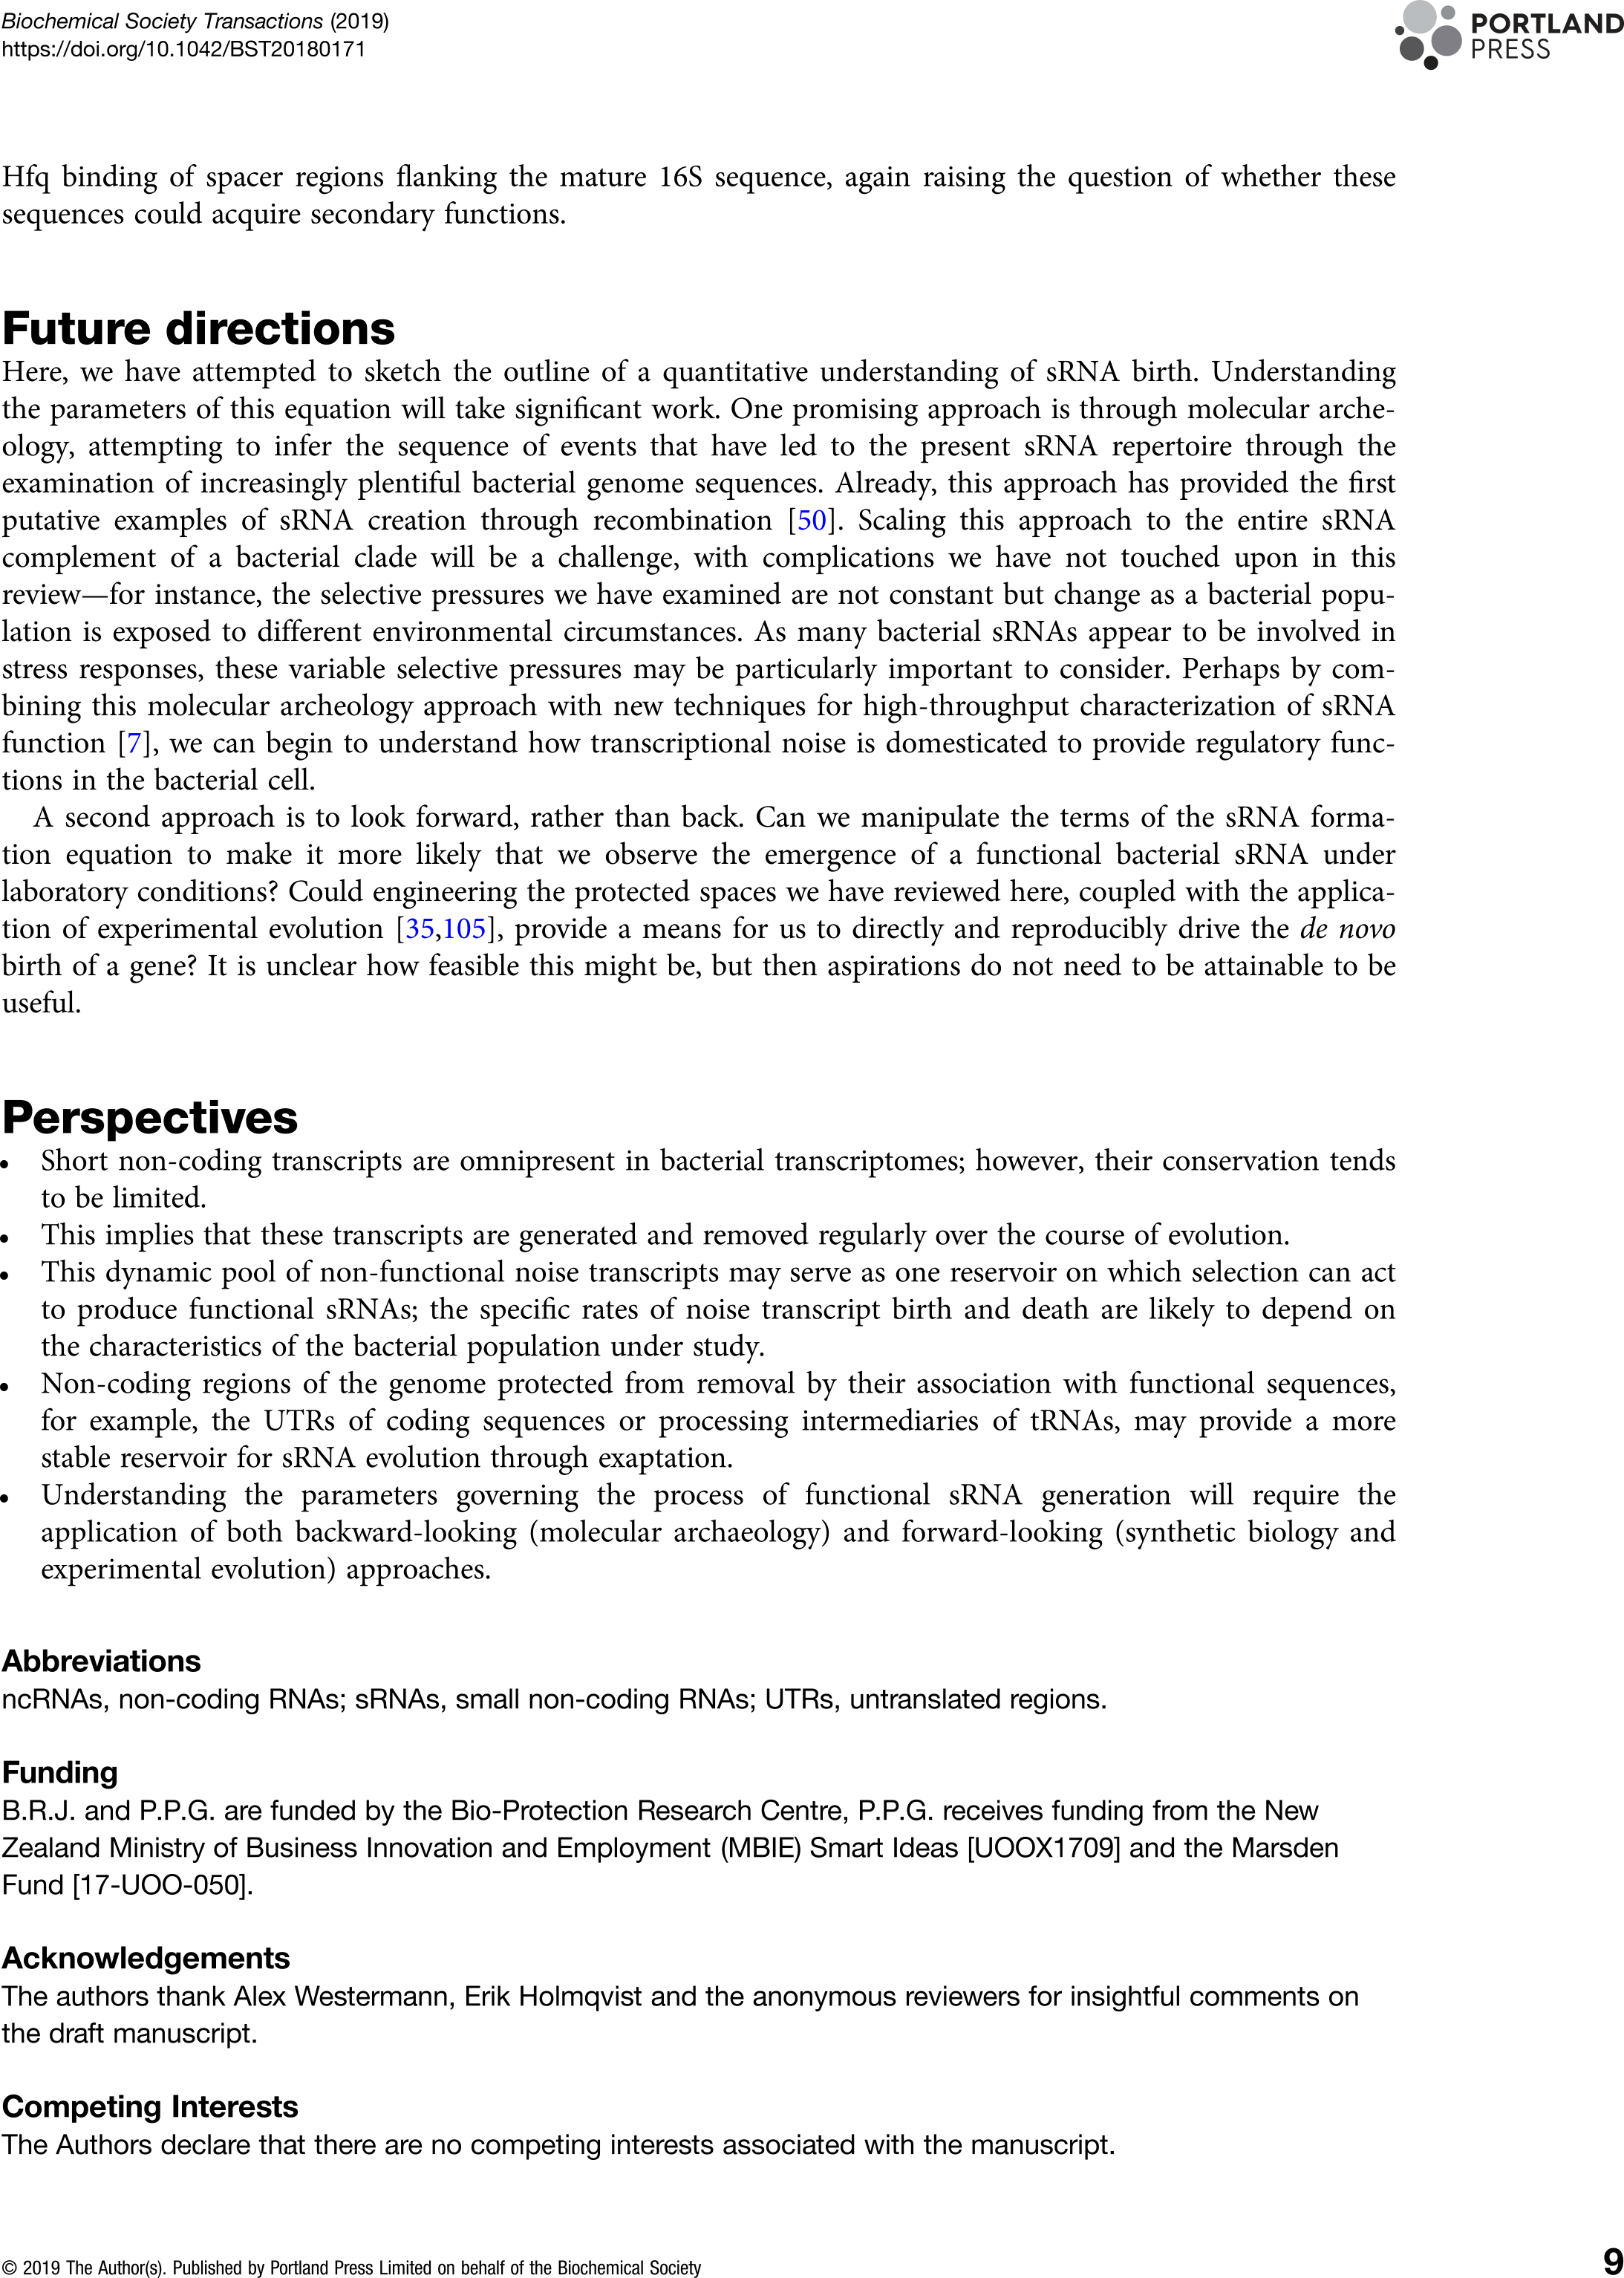
\includegraphics[width=\linewidth]{lit_review/page9.png}
\end{figure}
\begin{figure}
    \centering
    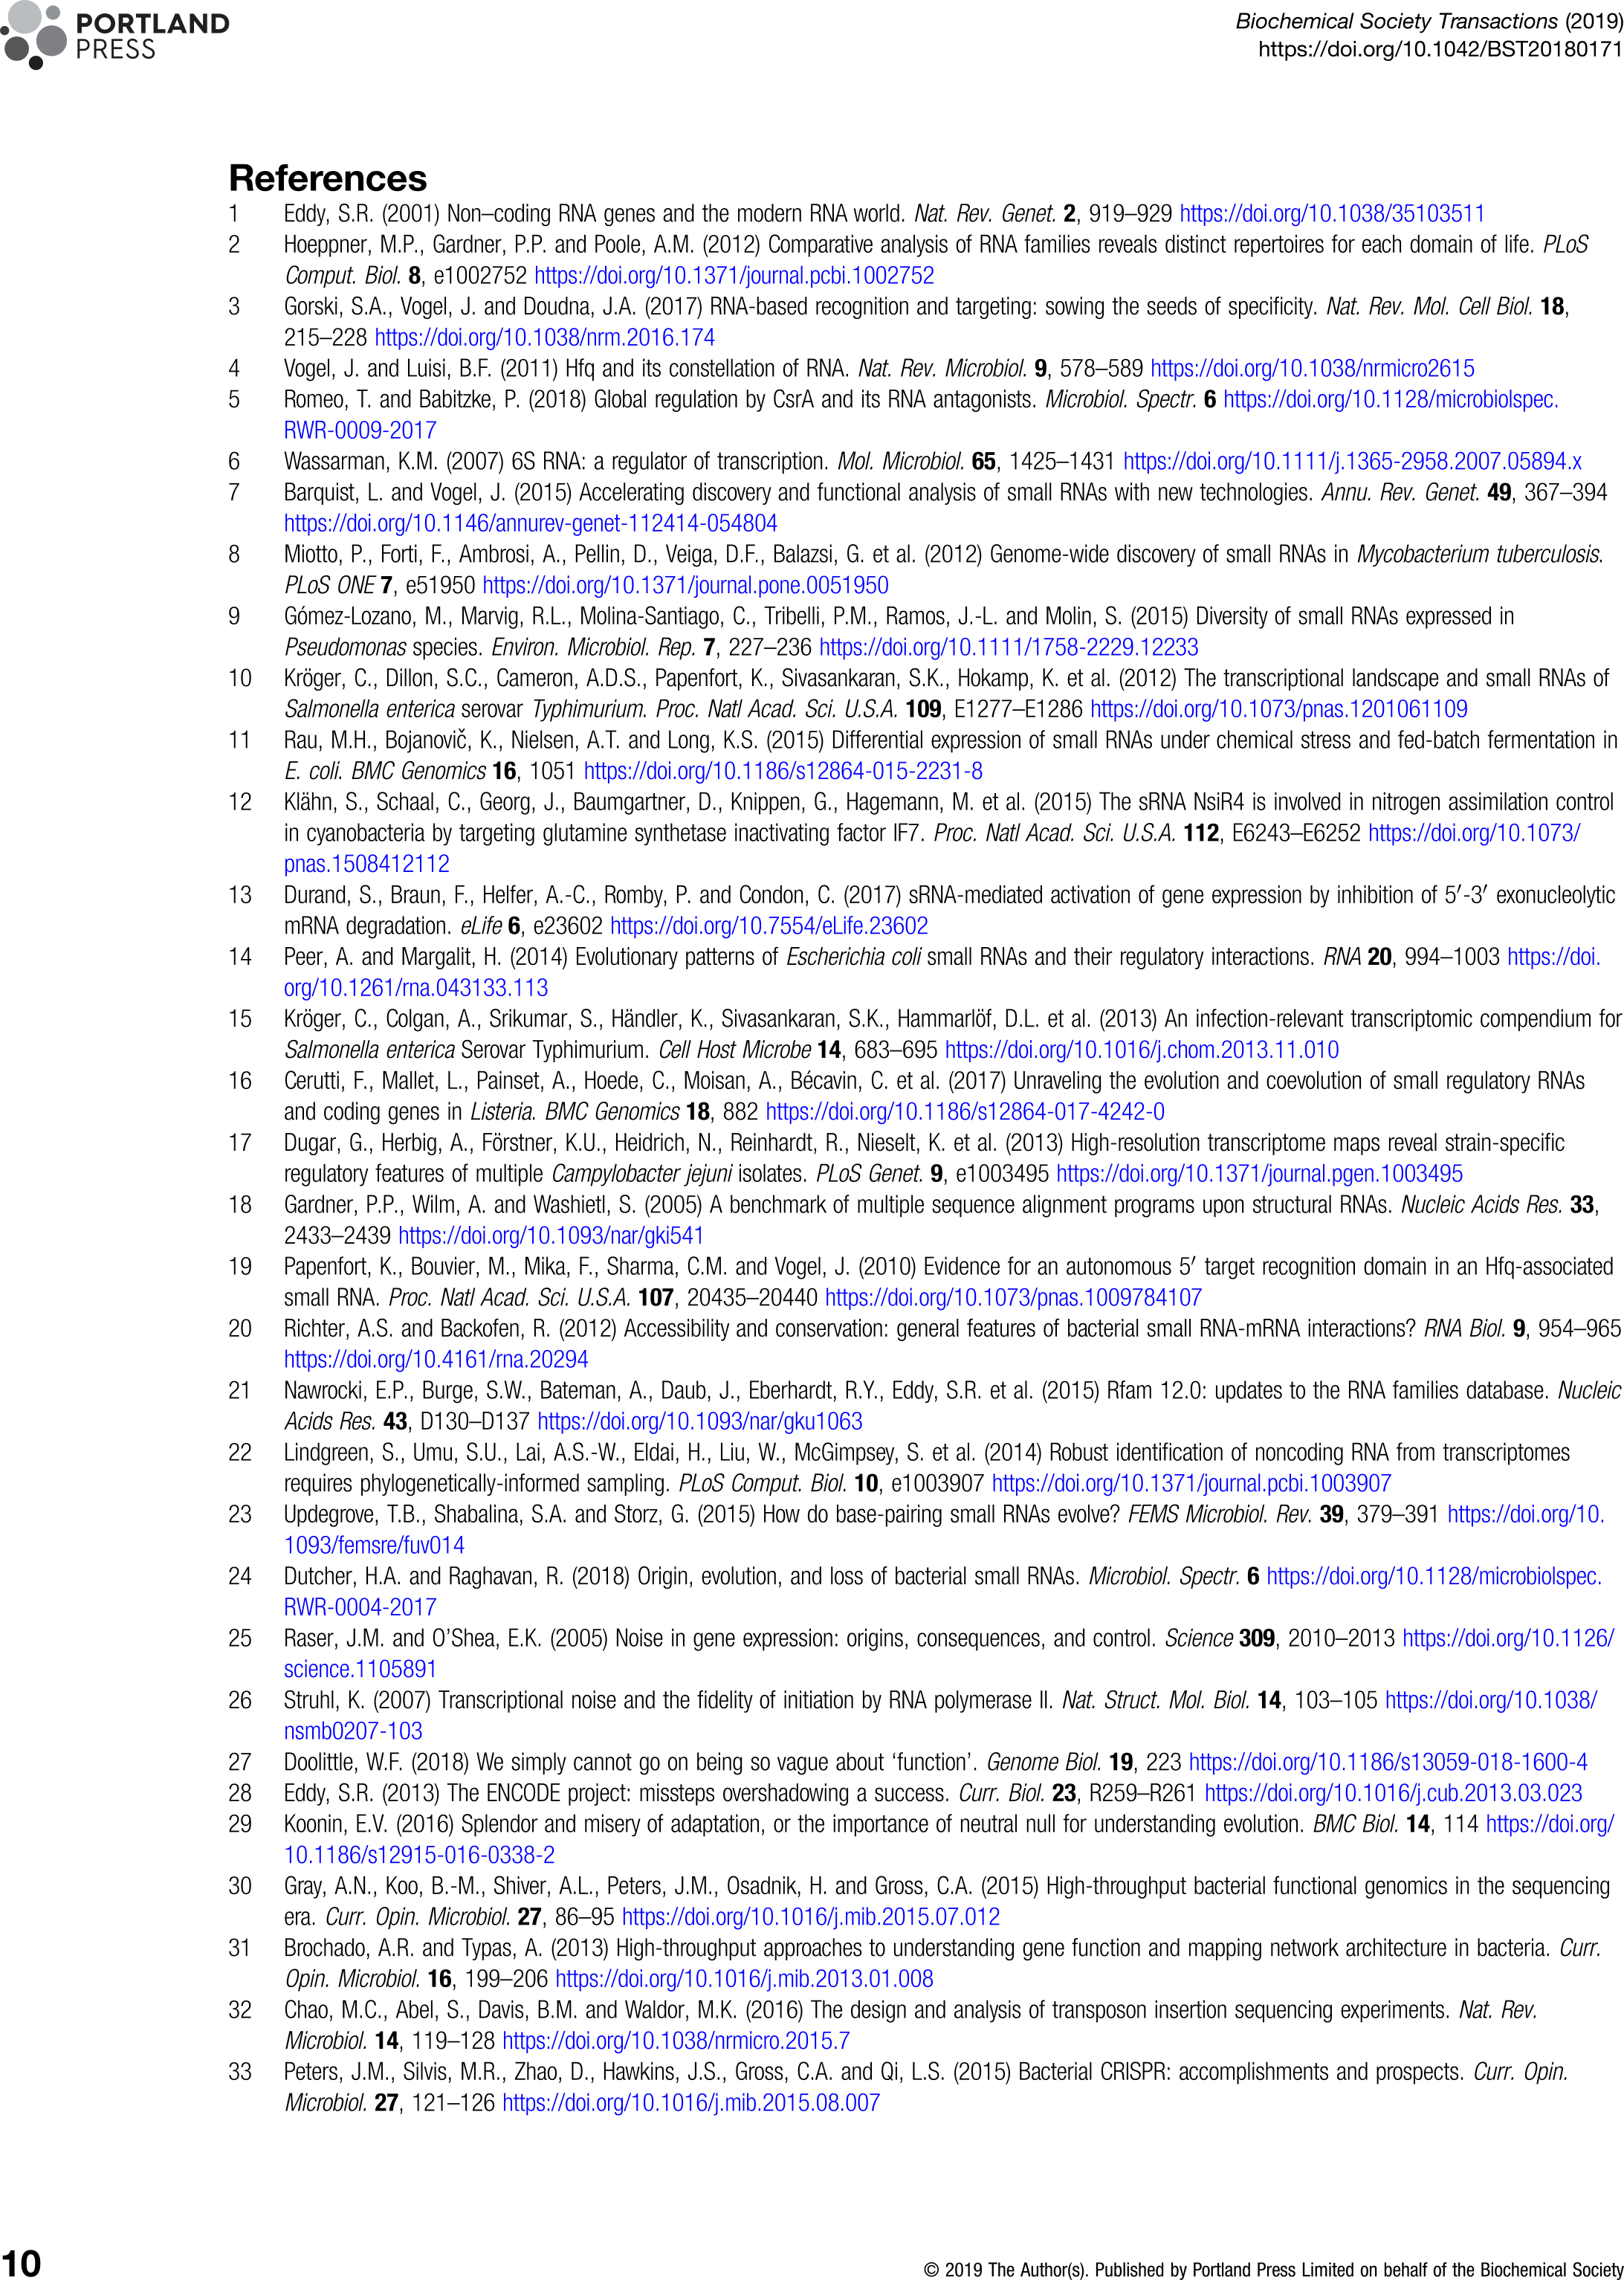
\includegraphics[width=\linewidth]{lit_review/page10.png}
\end{figure}
\begin{figure}
    \centering
    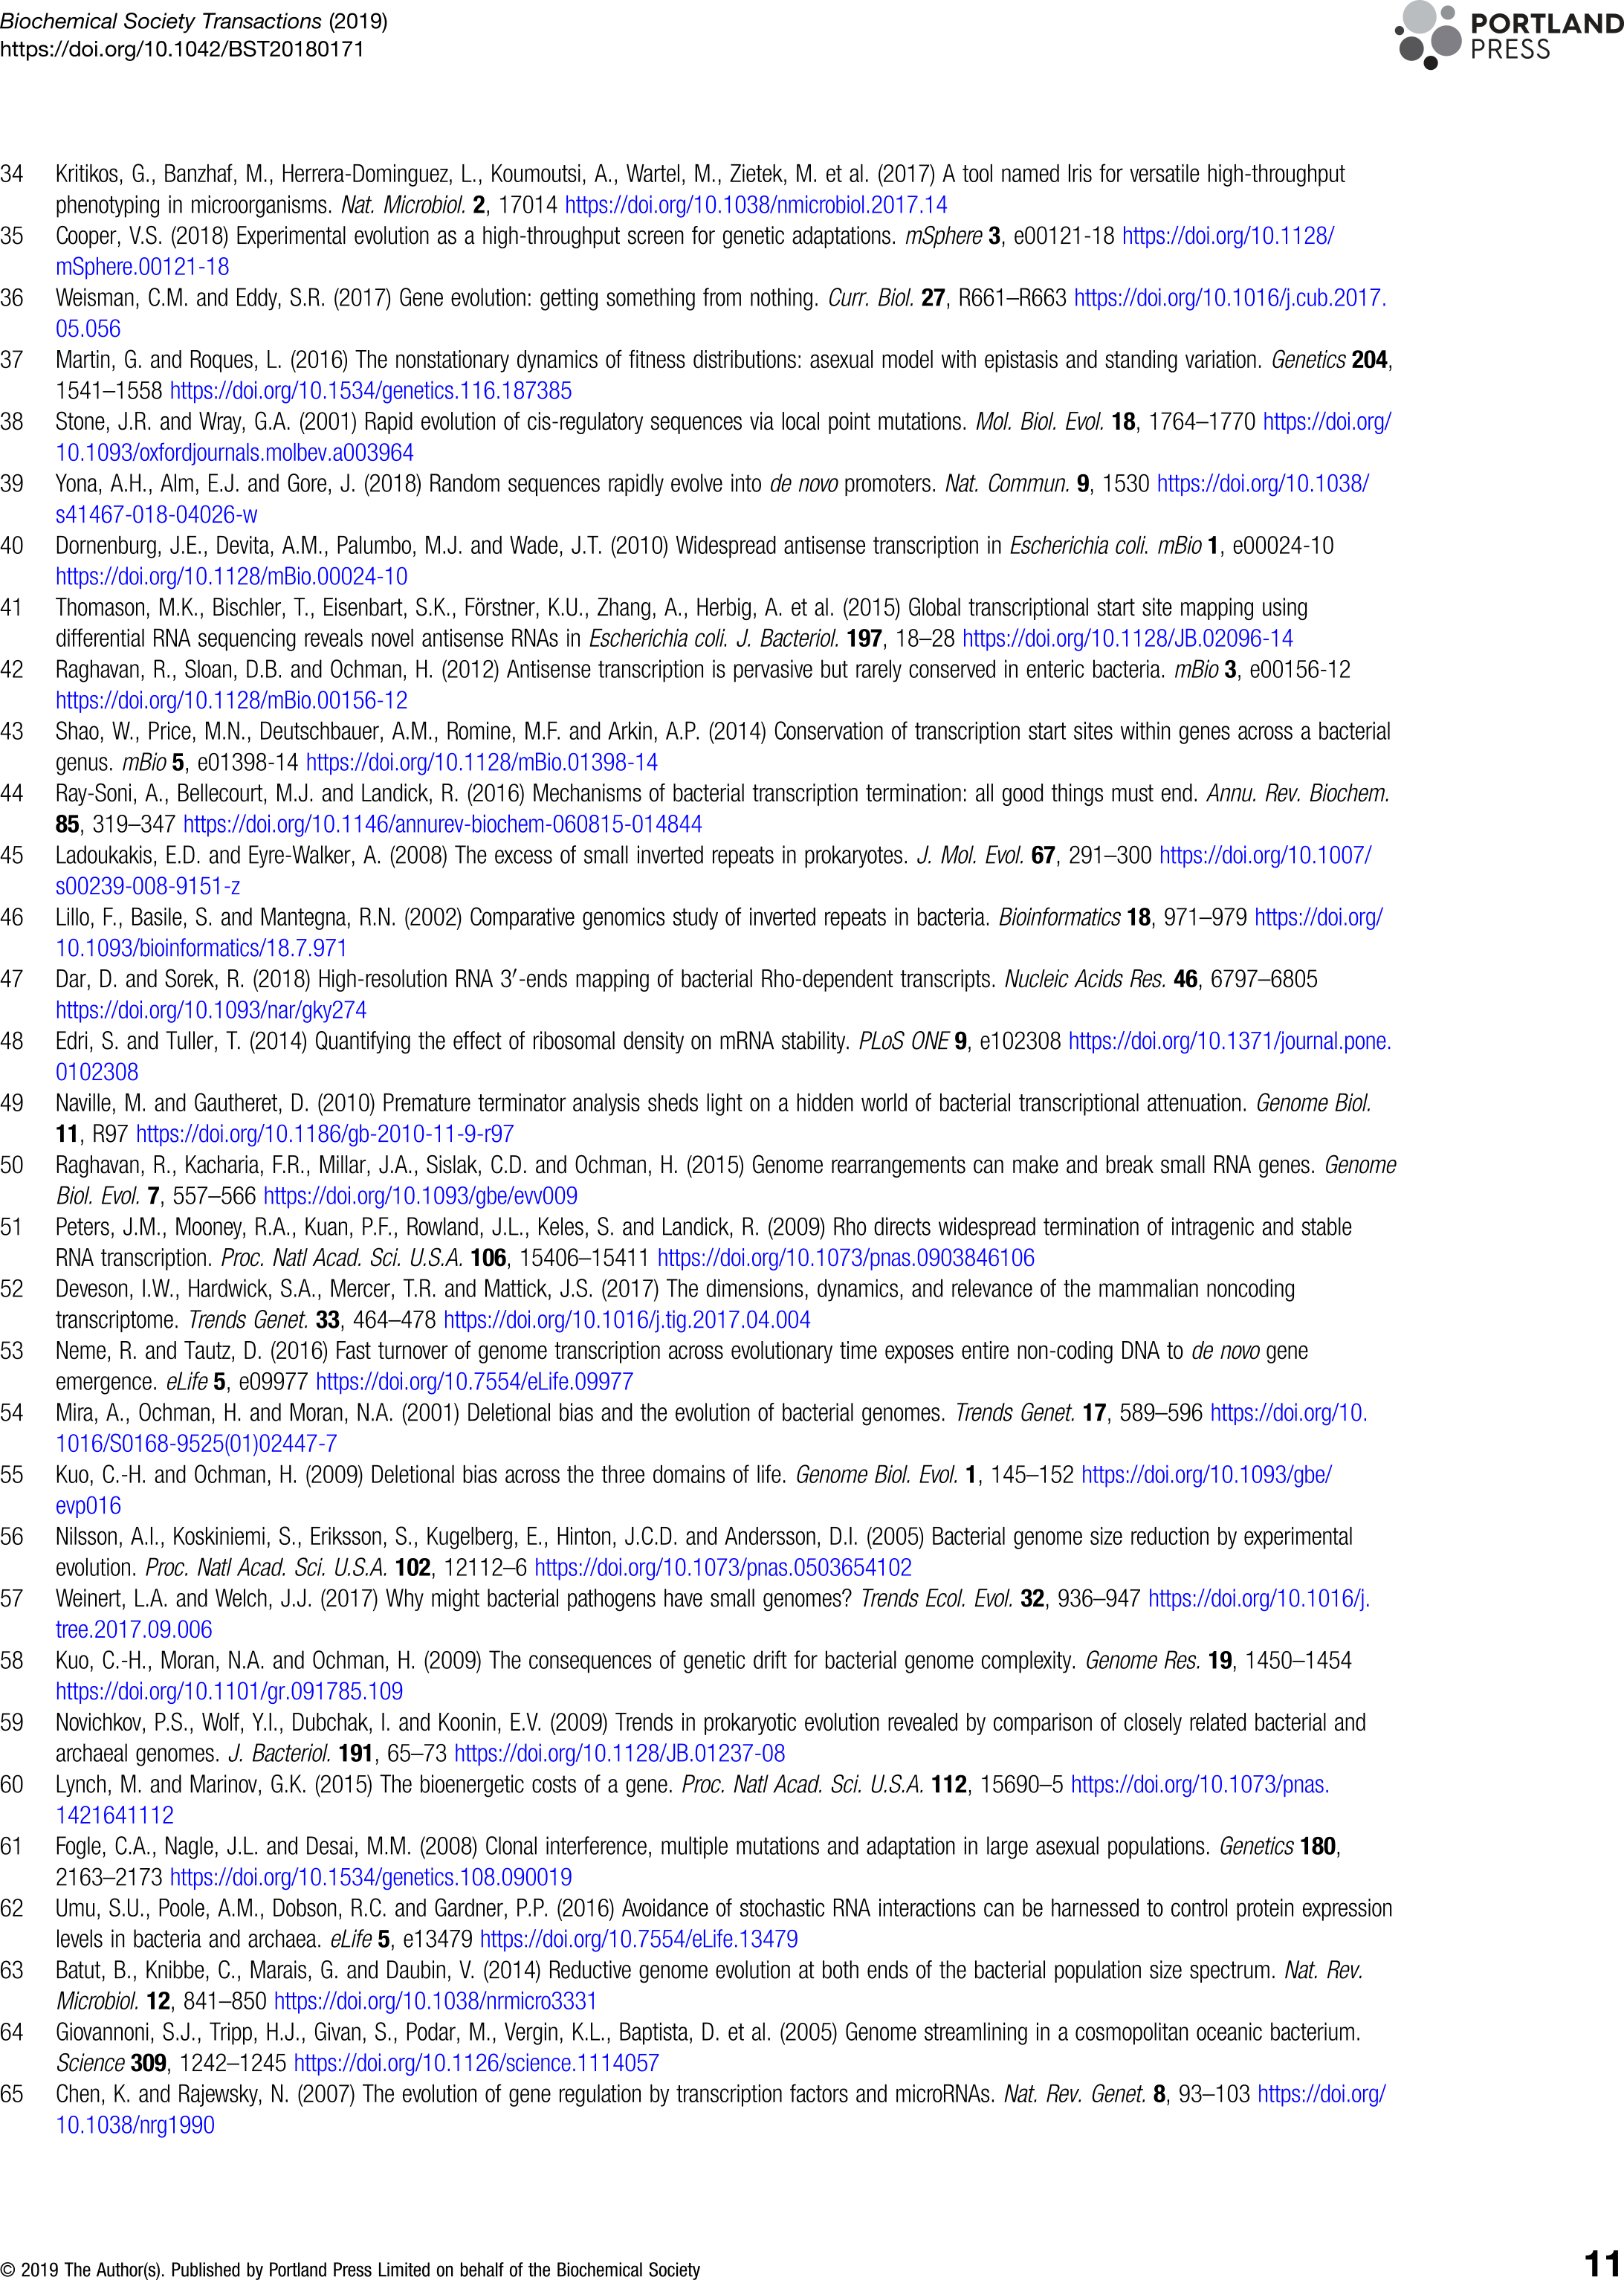
\includegraphics[width=\linewidth]{lit_review/page11.png}
\end{figure}
\begin{figure}
    \centering
    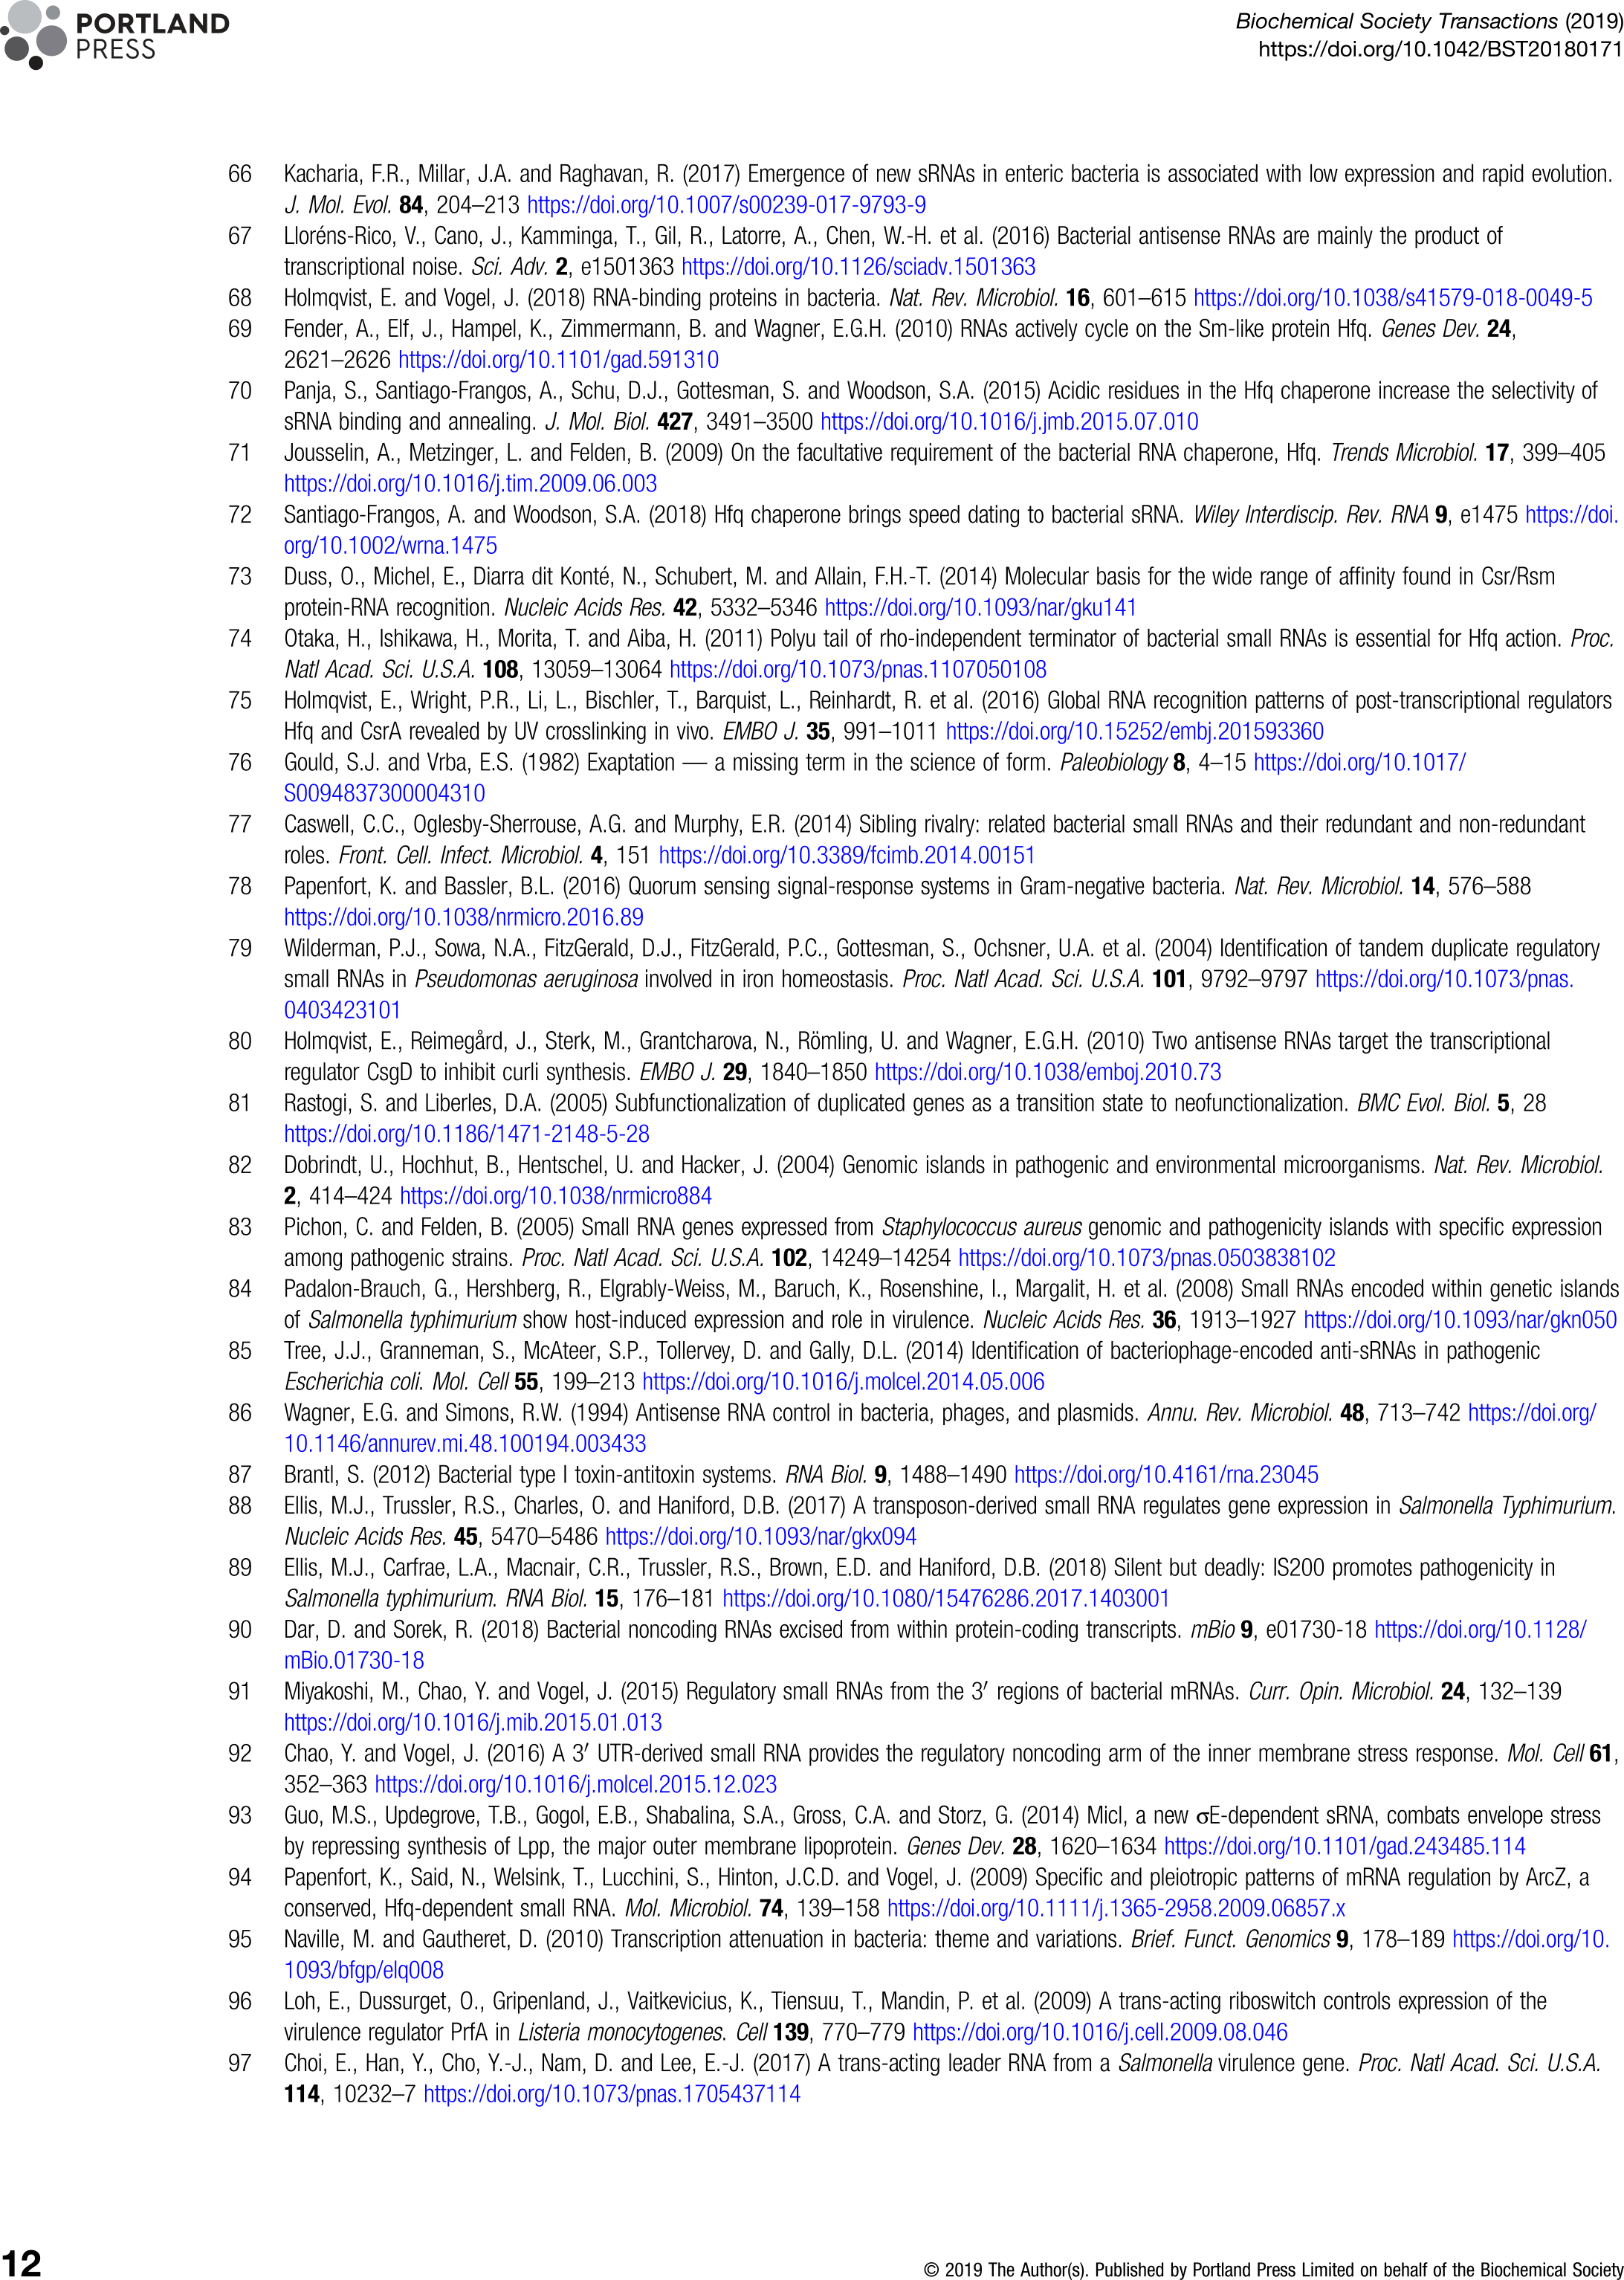
\includegraphics[width=\linewidth]{lit_review/page12.png}
\end{figure}
\begin{figure}
    \centering
    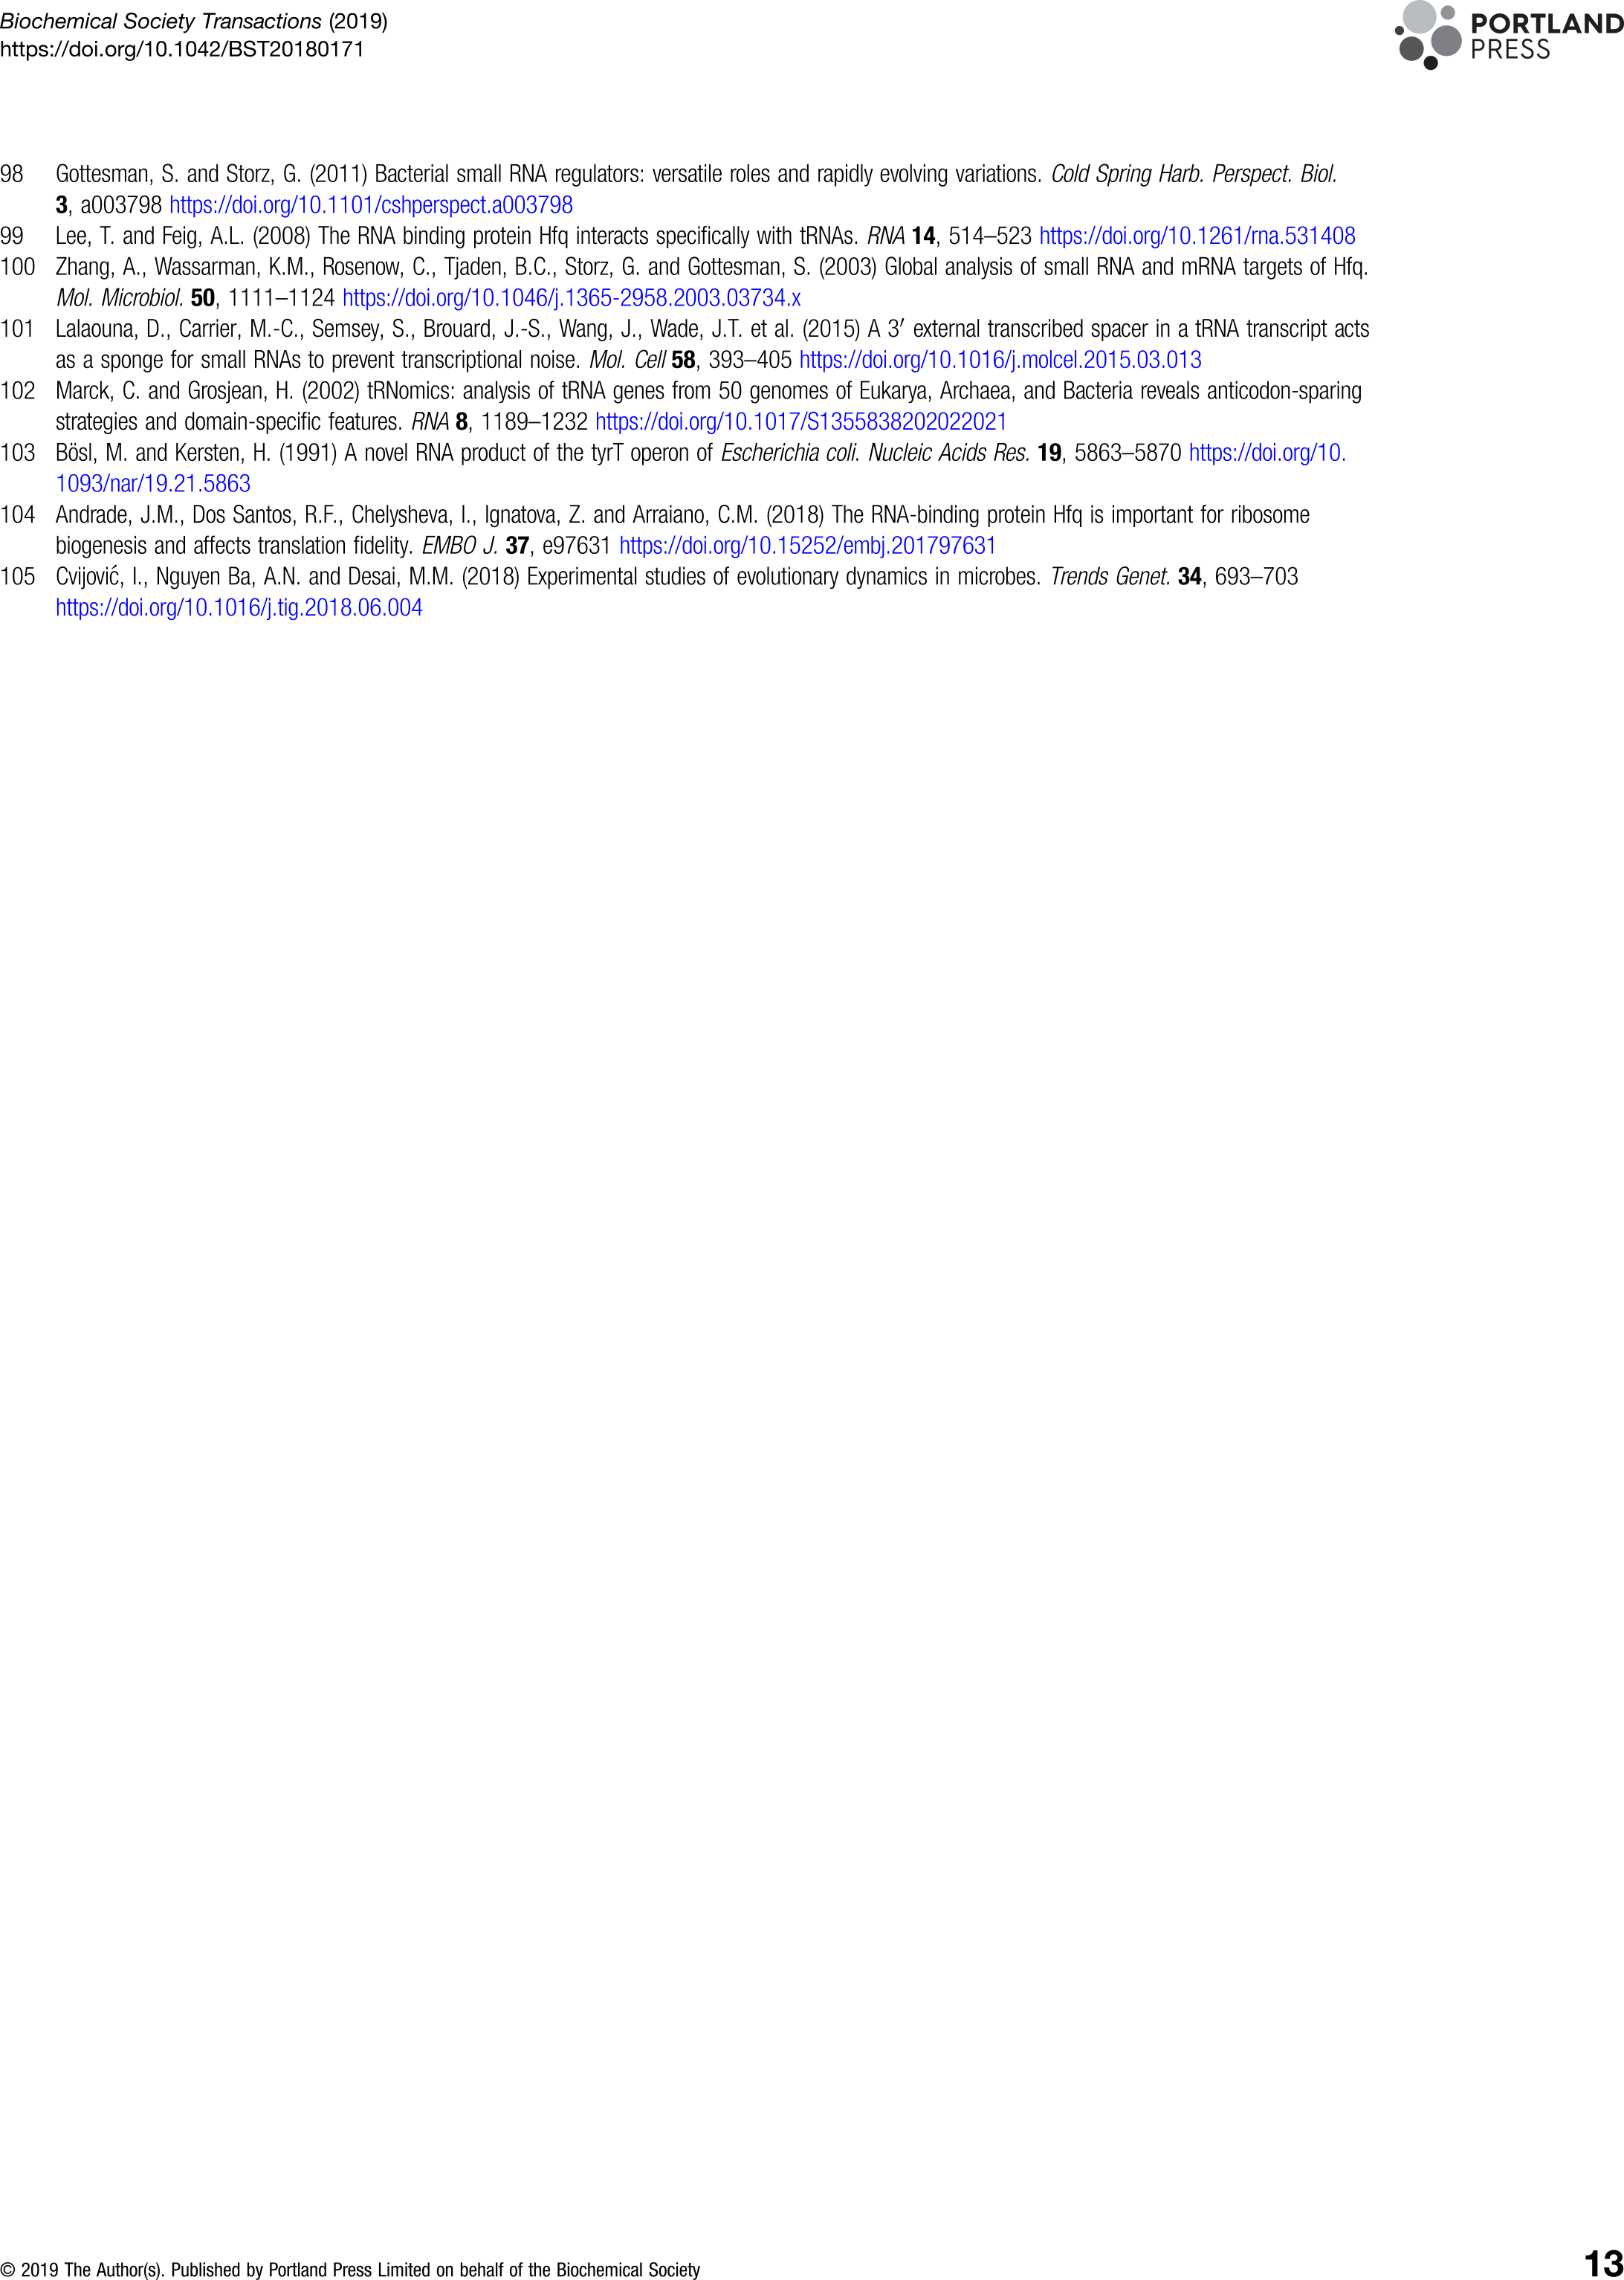
\includegraphics[width=\linewidth]{lit_review/page13.png}
\end{figure}